% Template for NAU "manuscript" style dissertation Mar 2023. Feel free to use with no guarantees or warranties.
\documentclass{book}
\usepackage[utf8]{inputenc}

\usepackage[bookmarks=true,
     pdfnewwindow=true,      % links in new window
     colorlinks=true,    % false: boxed links; true: colored links
     linkcolor=black,     % color of internal links; black to blue, 6/10/22 COC % black per NAU EDT 7/27/2022 COC
     citecolor=xlinkcolor,     % color of links to bibliography
     filecolor=xlinkcolor,  % color of file links
     urlcolor=xlinkcolor,      % color of external links
     final=true,
 ]{hyperref}


\usepackage[nointegrals]{wasysym}
\usepackage{siunitx}
\usepackage{mathtools} % loads amsmath also

\usepackage[letterpaper, portrait, margin=1in]{geometry}
\pagestyle{plain}
\raggedbottom  % CTU 22/12/12 get rid of space between paragraphs at end of chapters

\setcounter{secnumdepth}{3}

\usepackage{setspace}
\usepackage{lipsum}
\usepackage{float}
\usepackage{graphicx}
\usepackage{lscape}
\usepackage[printonlyused]{acronym}

\makeatletter
\newcommand*{\org@overidelabel}{}
\let\org@overridelabel\@verridelabel
\@ifpackagelater{acronym}{2015/03/21}{% v1.41
  \renewcommand*{\@verridelabel}[1]{%
    \@bsphack
    \protected@write\@auxout{}{\string\AC@undonewlabel{#1@cref}}%
    \org@overridelabel{#1}%
    \@esphack
  }%
}{% older versions
  \renewcommand*{\@verridelabel}[1]{%
    \@bsphack
    \protected@write\@auxout{}{\string\undonewlabel{#1@cref}}%
    \org@overridelabel{#1}%
    \@esphack
  }%
}
\makeatother

\acrodef{ac}{Acronym}

% \usepackage{amssymb} % leftrightsquiggle, etc.
\usepackage{textcomp,gensymb} % degree, etc. CTU 10/20/22

\usepackage{xcolor}
\definecolor{xlinkcolor}{cmyk}{0,0,0,1} % per NAU EDT 7/27/2022 COC
\PassOptionsToPackage{hyphens}{url}

\usepackage[percent]{overpic}
\usepackage{color}

% \usepackage{cleveref}
% \crefformat{footnote}{#2\footnotemark[#1]#3}

\usepackage{url}
\usepackage{natbib}
\bibliographystyle{aasjournal}  % Add different bib style .bst file if you'd like

\usepackage{enumitem}
\usepackage{makecell} % 12/27/2017 COC for multi-lined entries in tables
\usepackage{longtable} % spanning pages
\usepackage{multirow} % CJTU 12/15/22

% Wrapped figures and caption shenanigans 11/07/2022 CTU for inline figures
\usepackage[skip=5pt]{caption}
\DeclareCaptionFormat{boldtitle}
{%
    \textbf{#1#2} #3
}
\captionsetup{format=boldtitle,font={stretch=1.2}}
\usepackage{wrapfig} % for inline figures
\usepackage{etoolbox} % To fix misaligned wrapfigures
\BeforeBeginEnvironment{wrapfigure}{\setlength{\intextsep}{0pt}}
\BeforeBeginEnvironment{figure}{\setlength{\intextsep}{12.0pt plus 2.0pt minus 2.0pt}}

% Aliases
\newcommand{\dissertationTitle}{!YOUR TITLE ALL CAPS!}
\newcommand{\degr}{$\degree$}
\newcommand{\hho}{H$_2$O}
\newcommand{\ohhho}{OH / \hho}

%%%%%%%%%%%%
%me-
\usepackage[immediate]{silence}
\WarningFilter[temp]{latex}{Command} % silence the warnings from sectsy "\underbar has changed" "\underline has changed"
\usepackage{sectsty} % 6/26/2022 COC: control style of sectioning (e.g., font size) <- original line
\DeactivateWarningFilters[temp] % So nothing unrelated gets silenced

\makeatletter % disable the runtime redefinitions
\let\SS@makeulinesect\relax
\let\SS@makeulinepartchap\relax
\makeatother
%-me

% \allsectionsfont{\sffamily}
\chapternumberfont{\large}
\chaptertitlefont{\large}
\chapterfont{\large}
\allsectionsfont{\large}
\subsectionfont{\large}
\subsubsectionfont{\normalsize}
\paragraphfont{\normalsize}
% \sectionnumberfont{\large}
% \sectiontitlefont{\large}

%%%%%%%%%%%%%%%%%
\usepackage{calc}

\newcounter{rownumber}%12/26/2017 COC
%\renewcommand{\therownumber}{\thetable.\arabic{rownumber}}
%\newcounter{rtaskno}
%\newcommand{\rtask}[1]{\refstepcounter{rtaskno}\label{#1}}
\newcommand{\rlabel}[1]{\refstepcounter{rownumber}\label{#1}}
\setcounter{rownumber}{-36}

\newcounter{tabfoot}
\newcommand{\flabel}[1]{\refstepcounter{tabfoot}\label{#1}}
\renewcommand{\thetabfoot}{\alph{tabfoot}}
\setcounter{tabfoot}{-6}

\newcommand{\fakechapter}[1]{%
  \par\refstepcounter{chapter}% Increase chapter counter
%   \chaptermark{#1}% Add chapter mark (header)
  \addcontentsline{toc}{chapter}{\protect\numberline{\thechapter}#1}% Add section to ToC
}
\newcommand{\fakesection}[1]{%
  \par\refstepcounter{section}% Increase section counter
%   \sectionmark{#1}% Add section mark (header)
  \addcontentsline{toc}{section}{\protect\numberline{\thesection}#1}% Add section to ToC
}

\usepackage[figuresleft]{rotating} % forces all clockwise rotation per NAU EDT guidelines
\usepackage{pdflscape}  % CTU 11/18/22 use for landscape figures/tables

%%%%%%%%%%%%%%%%%%%%%%%%%%%%%%%%%%%%%%%%%%%%%%%%%%%%%%%%%%%%%%%%%%%%%%%%%%%
\begin{document}

%%%%%%%%%%%%%%%%%%%%%%%%%%%%%%%%%%%%%%%%%%%%%%%%%%%%%%%%%%%%%%%%%%%%%%%%%%%
\frontmatter  % Roman numerals
\begingroup  % Begin start chapter on any page
\let\cleardoublepage\clearpage  % Allow chapters to start on even pages
\doublespacing
  \begin{centering}
\begin{large}
\begin{spacing}{1.8}

\vspace*{\baselineskip}

\dissertationTitle{}

\thispagestyle{empty} % 4/28/2022 COC -- no page number on first page

\vspace{\baselineskip}

By Joel N. Johnson

% \vspace{10mm}

A Dissertation

Submitted in Partial Fulfillment

of the Requirements for the Degree of

% \vspace{10mm}

Doctor of Philosophy

in Applied Physics and Materials Science

\vspace{\baselineskip}

Northern Arizona University

!Month YYYY!

\vspace{2\baselineskip}

%Approved:

Ryan O. Behunin, Ph.D., Co-Chair

John G. Gibbs, Ph.D., Co-Chair

Inès Montaño, Ph.D.

Jennifer S. Martinez, Ph.D.

\end{spacing}
\end{large}
\end{centering}

  \phantomsection
\addcontentsline{toc}{chapter}{Abstract}

\begin{center}
    \large
    ABSTRACT

    \large
    \dissertationTitle{}

    \large
    \vspace{2mm}
    JOEL N. JOHNSON

\end{center}

% Abstract text max 350 words recommended
\noindent

This dissertation explores novel ways in which light and sound interact in optical waveguides to enable laser cooling of traveling-wave phonons and to enhance phonon spectroscopy. First, we establish how anti-Stokes Brillouin scattering can be harnessed to cool acoustic excitations in a continuous fiber, extending laser cooling concepts beyond discrete cavity optomechanical systems. By using a \ac{LCOF} filled with \ce{CS2}, we achieve significant reduction in the phonon population through spontaneous anti-Stokes processes. This demonstration marks the first instance of in-fiber traveling-wave phonon cooling without requiring nanophotonic resonators or specialized microstructures.

Second, we introduce a Coherently Stimulated Brillouin Spectrometer (\acs{CoBS}) that employs a four-wave mixing scheme—comprising pump, probe, driven Stokes, and observed signal fields—to dramatically improve sensitivity, especially for short, low-gain samples. By relaxing traditional phase-matching constraints, the CoBS approach enables sub-\SI{10}{\femto\watt} detection levels over millimeter- to centimeter-scale lengths. We validate its utility with measurements in both high- and low-gain media, opening new possibilities for ultrathin-film and microfluidic analyses.

Lastly, this dissertation investigates the theoretical and experimental conditions under which Brillouin-driven Raman-like modes might be observed. These “Brillouin-induced Raman” modes could provide a bridge between conventional Raman spectroscopy and the acousto-optic phenomena characteristic of traveling-wave phonons. While not yet fully realized, the groundwork here points to future avenues in which engineering the geometric and material properties of optical waveguides can yield both net phonon cooling and advanced hybrid phononic devices. Collectively, these results broaden our understanding of optomechanical coupling in fibers and pave the way for low-noise photonic systems, quantum acoustic memory elements, and highly sensitive, broadband spectroscopic tools.

  \include{pre/0-Copyright}
  \chapter*{Acknowledgements}
\phantomsection
\addcontentsline{toc}{chapter}{Acknowledgements}

%\textit{Note: Manuscript-specific acknowledgements are found at the end of each corresponding chapter.}
%\section*{In Memoriam}
%\section*{Individuals and Groups}
%\section*{Funding}
%\section*{General Acknowledgements}

%Lauren

%Parents

%Gibbs: Live long and prosper, friend

%Research group: Gabe, V, Dylan, Dani

%friends: Josh, Tyler, Derek, others


%%%%%%%%%%%%%%%%%%%%%%%%%%%%%%%%%%%%%%%%%%%%%%%%%%%%%%%%%%%%%%%%%%%%%%%%%%%
\singlespacing
\setcounter{tocdepth}{3} % depth of sections diplayed in table of contents
\renewcommand{\contentsname}{Table of Contents}
\tableofcontents
\doublespacing

%%%%%%%%%%%%%%%%%%%%%%%%%%%%%%%%%%%%%%%%%%%%%%%%%%%%%%%%%%%%%%%%%%%%%%%%%%%
\clearpage
\phantomsection
\addcontentsline{toc}{chapter}{List of Tables}
\listoftables

%%%%%%%%%%%%%%%%%%%%%%%%%%%%%%%%%%%%%%%%%%%%%%%%%%%%%%%%%%%%%%%%%%%%%%%%%%%
\clearpage
\phantomsection
\addcontentsline{toc}{chapter}{List of Figures}
\listoffigures
\endgroup  % End start chapter on any page
\doublespacing

%%%%%%%%%%%%%%%%%%%%%%%%%%%%%%%%%%%%%%%%%%%%%%%%%%%%%%%%%%%%%%%%%%%%%%%%%%%
\chapter*{Dedication}
\phantomsection
\addcontentsline{toc}{chapter}{Dedication}


%%%%%%%%%%%%%%%%%%%%%%%%%%%%%%%%%%%%%%%%%%%%%%%%%%%%%%%%%%%%%%%%%%%%%%%%%%%
\chapter*{Preface}
\phantomsection
\addcontentsline{toc}{chapter}{Preface}
% For manuscript style chapters, NAU wants a preface describing what's to follow


 %This dissertation consists of five chapters: Introduction (\autoref{chap:intro}), three manuscript chapters (\autoref{chap:spweather}, \autoref{chap:roughness}, \autoref{chap:moonpies}), and the Discussion \& Conclusion (\autoref{chap:discussion}). Chapters \ref{chap:spweather}--\ref{chap:moonpies} were prepared as manuscripts to appear in peer-reviewed scientific journals. As of this writing, \textit{\nameref{chap:spweather}} was published as \cite{taiudovicic2021} in Geophysical Research Letters (doi: \url{https://doi.org/10.1029/2020GL092198}), chapter \textit{\nameref{chap:moonpies}} was recently submitted to a journal for peer review, and chapter \textit{\nameref{chap:roughness}} is being prepared for submission. During the review process, the contents of Manuscript II and III may change such that their published versions differ from the contents of \autoref{chap:roughness} and \autoref{chap:moonpies}, respectively. Additionally, there may be some redundancy in the contents of the three manuscript chapters which were written to appear as standalone works in the literature.


%%%%%%%%%%%%%%%%%%%% INTRO & METHODS %%%%%%%%%%%%%%%%%%%%%%%%%%%%%%%%%%%%%%
\mainmatter  % Regular numbers
\chapter{Introduction}
\label{ch:Introduction}
\acresetall

%TOO SELF INTERESTED! State facts
%The work presented in this document details my efforts toward achieving a result for which my time and available resources would prove too limited to accomplish in full. It is my great hope that a dear future reader may someday be inspired to take up where I left off and realize the result that I have been chasing for these years. No physical principle disallows the demonstration of this result, only practical challenges stand in its way.

%The physics involved in this research effort primarily lies in the field of optomechanics, however it veers at times into the related domains of nonlinear optics and nanoscience. I have in fact developed a great love for each of these fields and it was my romantic goal to unite them that originally led me to pursue this work. In this introductory chapter I present the foundational topics and concepts that I employ in later chapters.

Optomechanics is the study of light-matter interactions; it is the study of how the intangible (light) can affect change in the tangible (matter) and vice versa. Injecting light into a material under specific conditions allows for an exchange of energy to occur between the light and the mechanical oscillations of the material which changes the mechanical energy of the material. This interaction can be controlled to deposit or withdraw mechanical energy into/from a system and thus leave the system in a more, or less, mechanically energetic state respectively. The same interaction can also be harnessed for passive observation of material properties. Mechanical systems from bulk to atomic scales can be probed and characterized with light by retrieving the inelastically scattered light resulting from interaction with the material. This retrieved light contains embedded information about the energy exchange that occurred, which, when considered as part of a population of scattering events, reveals natural resonances of a mechanical system.

Optomechanics comprises a broad range of phenomena involving the interaction of optical and mechanical systems, from basic photothermal absorption to more complex nonlinear processes. Here I offer a brief overview of notable optomechanical phenomena then devote the remainder of this chapter to a more detailed description of the specific interactions that play a role in my research. Photothermal absorption is the process by which light is absorbed by a material, leading to an increase in temperature of the material and consequent changes in the material's dimensions (thermal expansion) or refractive index (thermo-optic effect). This effect has applications in optical switches\cite{}, actuators\cite{}, and sensors\cite{}. Photothermal therapy in medicine is an emerging application of this effect, where light is used to target and heat specific areas, causing localized damage to diseased tissue\cite{}. This technique becomes especially effective when combined with nanoparticle-enhanced absorption, allowing for dramatically increased absorption in ultra-localized zones within the body.

Light scattering, in its many forms, is also an optomechanical process as it involves the interaction of an optical field with the fluctuation, motion, or vibration of matter. Rayleigh scattering, perhaps the most well-known example, is the elastic scattering of light by particles much smaller than the wavelength of the incident light, leading to scattering in possibly a new direction but without a change in wavelength. It is responsible for the blue color of the sky because the efficiency of Rayleigh scattering is inversely proportional to the fourth power of the wavelength ($\lambda$) of the light ($\frac{1}{\lambda^{4}}$) and so shorter (blue) wavelengths are scattered much more than longer (red) wavelengths by the molecules in the atmosphere.\cite{rayleigh1871light}

Raman scattering is the interaction of light with vibrational and rotational modes within a material (often molecular), resulting in scattered light with frequencies that are shifted from the incident light. This inelastically scattered light provides insights into the material's molecular structure and properties. Raman scattering is widely used in chemical and material science for identifying chemical compounds, analyzing molecular structures, and studying molecular dynamics. It finds application in the characterization of pharmaceuticals\cite{}, monitoring changes in biological tissues for medical diagnostics\cite{}, and investigation of stress and temperature distributions in engineering materials\cite{}, among others\cite{}.

Brillouin scattering, around which much of my work is centered, is the scattering of light with acoustic phonons or coherent traveling density waves in a material, resulting in scattered light with a frequency that is slightly shifted from the incident light. This inelastically scattered light reveals mechanical properties of the material such as its bulk and elastic moduli. This phenomenon is used in materials science to measure elastic properties and viscoelasticity of materials\cite{}, in fiber optic sensing to monitor temperature and strain over large distances\cite{}, and in physics to study phase transitions and mechanical properties of crystals, liquids, and gases\cite{}.

Rayleigh-wing scattering is the broad, smooth extension of the Rayleigh scattering spectrum that results from interactions with low-frequency excitations in a material, providing insights into dynamic processes like rotational and translational diffusion of molecules that make up a material. This scattering is particularly useful in studying the dynamics of complex fluids, gases, and soft materials, where it can reveal information about molecular orientation, diffusion rates, and interactions within the medium. Applications include the analysis of atmospheric phenomena\cite{}, characterization of liquid crystals\cite{}, and investigations into the properties of polymers and biological materials\cite{}, aiding in the understanding of their behavior at the molecular level.

Figure \ref{fig:Introduction:scattering-domains} shows the relative domains of typical frequency shifts for Rayleigh, Rayleigh-wing, Brillouin, and Raman scattering. Rayleigh-wing scattering is broad and shares part of its domain with Brillouin scattering. This makes sense because for any given molecule and within the timescale that it occurs, diffusive translational motion can be thought of as indistinguishable from motion caused by traveling density waves that host brillouin scattering. In this way, Rayleigh-wing scattering represents a sporadic distribution of fleeting, localized Brillouin scattering. Of course, the difference between incoherent diffusion of molecules and coherently traveling acoustic modes within a material is an important distinction. However, this thought experiment offers a perspective for bridging the gap between Rayleigh-wing and Brillouin scattering and for understanding their common frequency domains. Moreover, it serves as a reminder of the rich continuum of material behavior and responses that affect light scattering as opposed to the distinct categories we ascribe for convenience. This is a core concept of my work.%Boyd 9.6 works out general theory of Brillouin and Rayleigh scattering!

% This makes sense, as the [random and incoherent] translational motion of molecules as they [continuously] diffuse [according to the laws of thermodynamics and as described by statistical mechanics] can be thought of, within the timescale that this motion occurs, as indistinguishable from [translational motion as caused by coherent] traveling density waves which host brillouin scattering.

\begin{figure}[t] % here (h), at the top (t), at the bottom (b), or on a separate page for floats (p), in that preference order
\centering
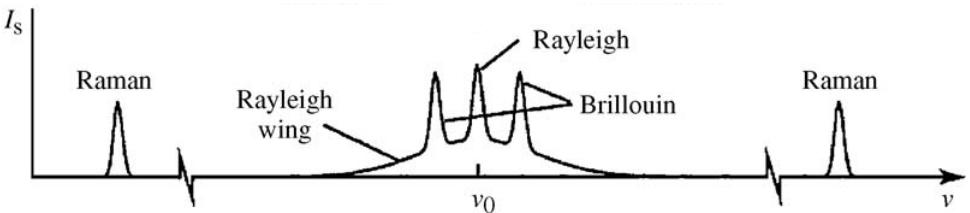
\includegraphics[width=0.75\linewidth]{figs/1-Intro/Boyd scattering frequency shift domains.png}
\caption{Relative domains of typical frequency shifts for Rayleigh, Rayleigh-wing, Brillouin, and Raman scattering.}
\label{fig:Introduction:scattering-domains}
\end{figure}

Returning to other optomechanical phenomena beyond scattering processes, the momentum of photons can exert forces on objects, leading to phenomena like radiation pressure, optical tweezing, and optical trapping. These effects are widely used in manipulating microscopic particles\cite{}, biological cells\cite{}, and atoms\cite{}, enabling studies of single molecules\cite{}, cold atoms\cite{}, and quantum computing elements\cite{}.

The final category of optomechanical interactions I will note here is that of nonlinear optical phenomena. Second harmonic generation, parametric oscillation, and four-wave mixing all feature the interaction between light and material nonlinearities that lead to the generation of new light frequencies.\cite{boyd2020nonlinear} The Kerr effect is the change in the refractive index of a material in response to an applied electric field, which can be induced optically with sufficient intensities of light. In general, nonlinear optical responses of materials are often only accessible with the use of high intensity laser light. This is emphasized by the fact that the field of nonlinear optics can be traced back to the discovery of second-harmonic generation in 1961\cite{franken1961generation}, just one year after the first demonstration of the laser by American physicist Theodor Maiman.\cite{maiman1960stimulated} These nonlinear effects provide the foundation for a range of technologies, including high-speed optical communication systems\cite{}, frequency converters\cite{}, and lasers for materials processing\cite{}.

Also included within nonlinear optical phenomena is electrostriction. Electrostriction is a reversible material deformation induced by an electric field, which can be generated by light in electro-optic materials. This effect is quadratic, scaling with the square of the applied electric field, and hence a nonlinear optical effect. At sufficiently high intensities, electrostrictive forces serve to enhance Brillouin scattering whereby the scattered light electrostrictively reinforces the acoustic wave that caused its scattering, leading to a nonlinear positive feedback loop known as \ac{SBS}. Photostriction is a related phenomenon that occurs when light absorption causes a change in the lattice structure of a material, leading to mechanical strain. It combines photovoltaic and piezoelectric effects and can be seen as an optically induced strain. These effects are utilized in designing optical modulators\cite{}, tunable photonic devices\cite{}, and smart materials that respond to light\cite{}.

In the remainder of this chapter I further describe the specific optomechanical phenomena that pertain to the research presented in this document: Brillouin scattering, electrostriction as it pertains to the \ac{SBS} process, and Raman scattering.


%%%%%%%%%%%%%%%%%%%%%%%%%%%%%%%%%%%
\section{Light Scattering}
\label{sec:Introduction:Light-Scattering}
Light scattering involves the redirection of light as a result of interactions with the constituent particles or molecules within a material medium. In every case, light scattering occurs because of variations in the material's optical properties. To understand why, envision a material with completely uniform particles---spatially and temporally consistent, or in other words, perfectly homogeneous. Figure \ref{fig:Introduction:homogeneous-material-no-scatter} shows an incident optical plane wave encountering a segment of such a material, denoted $\delta z$, containing a volume element $\delta V_{1}$. For any given incident wavelength $\lambda$ and any non-zero scattering angle $\theta$ at volume $\delta V_{1}$, there exists a corresponding volume element $\delta V_{2}$, located a distance $\frac{\lambda}{2\sin\theta}$ apart, which scatters light at the same angle $\theta$. The scattered waves from $\delta V_{1}$ and $\delta V_{2}$ would be out of phase by $\frac{\lambda}{2}$, leading to perfect destructive interference and no resultant scattered field. Thus, to achieve observable scattering, the material must possess inhomogeneities, allowing for variations in the optical properties between neighboring volumes. Fortunately, perfect homogeneity is not characteristic of real materials; all matter undergoes thermodynamic fluctuations at any temperature above absolute zero, and quantum fluctuations are inherent even at the ground state.

I now begin with a theoretical description of spontaneous light scattering as a result of thermodynamic fluctuations, presented in Boyd Nonlinear Optics.\cite{boyd2020nonlinear} This foundation will serve as a framework for understanding light scattering as specifically resulting from pressure variations (Brillouin scattering) as opposed to density variations (Rayleigh scattering). Later I will treat the case of higher-intensity \ac{SBS}. Ultimately I will build upon this theoretical basis to derive the coupled-wave equations of \ac{CABS}, a novel instrument which underpins many of my results. Let us build a theoretical description of light scattering considering thermodynamic fluctuations as the origin of the scattering process.

\begin{figure}[t] % here (h), at the top (t), at the bottom (b), or on a separate page for floats (p), in that preference order
\centering
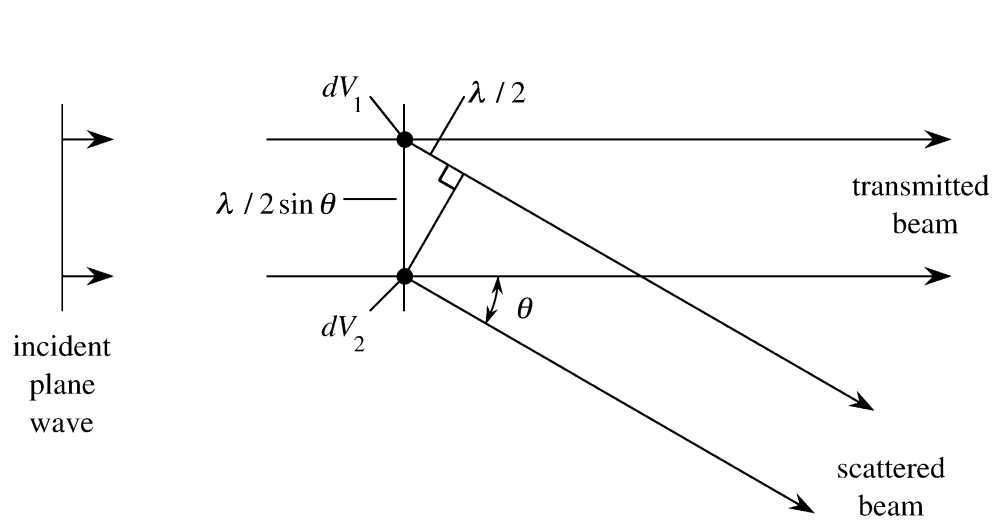
\includegraphics[width=0.75\linewidth]{figs/1-Intro/Boyd homogeneous material no scatter.png}
\caption{}
\label{fig:Introduction:homogeneous-material-no-scatter}
\end{figure}

\section{Spontaneous Brillouin Scattering}
\label{sec:Introduction:Spontaneous-Brillouin}
\lipsum[1]

\section{Stimulated Brillouin Scattering}
\label{sec:Introduction:Stimulated}
\lipsum[1]

\section{Phase-matching}
\label{sec:Introduction:Phase-matching}
\lipsum[1]

\section{Brillouin Gain of Materials}
\label{subsec:Introduction:Gain}
\lipsum[1]

\section{Raman Scattering}
\label{sec:Introduction:Raman}
\lipsum[1]

\section{Raman-like Brillouin Modes}
\label{sec:Introduction:Raman-like}
\lipsum[1]


%%%%%%%%%%%%%%%%%%%%%%%%%%%%%%%%%%%%%%%%%%%%%%%%%%%%%%%%%%%%%%%%%%%%%%%%%%%

\chapter{Foundational Experimental Techniques and Instrumentation}
\label{ch:Experimental}
\acresetall

This is an inline citation, \cite{boyd2020nonlinear}. This is a parenthetical citation \citep{boyd2020nonlinear}. This is a figure reference (Figure \ref{fig:Introduction:scattering-domains}). This is a section reference \S\ref{sec:Introduction:Spontaneous-Brillouin}. This is a chapter reference with chapter spelled out: \autoref{ch:Cooling}. This is an acronym definition \ac{AGU}. This is the second time I use the acronym in this section \ac{AGU}. This is if I want to spell out the full acronym again \acf{AGU}. Define new acronyms in the acronyms.tex file.

%--------------------------------------------------------------------%

\section{Photonic Experimental Techniques}
\label{sec:Experimental:Experimental Techniques}


\subsection{Control of Light in Photonic Systems}
\label{subsec:Experimental:Techniques:Control}


\subsection{Photonic Devices and Diagrams}
\label{subsec:Experimental:Techniques:Diagrams}


\subsection{Selection and Isolation of Signals}
\label{subsec:Experimental:Techniques:Signals}


\subsection{Heterodyne Detection and the Local Oscillator}
\label{subsec:Experimental:Techniques:Heterodyne}


\subsection{Optical Loss in a Photonic Systems}
\label{subsec:Experimental:Techniques:Loss}


\subsection{Free Space Optics and Beam Alignment}
\label{subsec:Experimental:Techniques:Alignment}


\subsection{Specialized Optical Fibers}
\label{subsec:Experimental:Techniques:Fibers}

%--------------------------------------------------------------------%

\section{Optical Instrumentation}
\label{sec:Experimental:Optical Instrumentation}

%--------------------------------------------------------------------%

\section{Electronic Instrumentation}
\label{sec:Experimental:Electronic Instrumentation}

%--------------------------------------------------------------------%

\section{Noise and Background Handling}
\label{sec:Experimental:Noise}

%--------------------------------------------------------------------%

\section{Custom Software}
\label{sec:Experimental:Software}


\subsection{Description of Python Script for CABS Data Collection}
\label{subsec:Experimental:Software:Python}


\subsection{Description of Plotting Data in Go Program}
\label{subsec:Experimental:Software:Go}


%%%%%%%%%%%%%%%%%%%% MANUSCRIPT CHAPTERS %%%%%%%%%%%%%%%%%%%%%%%%%%%%%%%%%%
\clearpage
\setcounter{rownumber}{0}
\chapter{Manuscript I: Laser cooling of traveling wave phonons in an optical fiber}
\label{ch:Cooling}
\acresetall

%--------------------------------------------------------------------%

\section{Abstract}
\label{sec:Cooling:Abstract}

%--------------------------------------------------------------------%

\section{Optomechanical Cooling and Heating}
\label{sec:Cooling:Cooling-Heating}

%--------------------------------------------------------------------%

\section{Cooling Platform: \texorpdfstring{$CS_{2}$}{CS2}-Liquid Core Optical Fiber}
\label{sec:Cooling:Platform}


\subsection{Optomechanical Properties}
\label{subsec:Cooling:Platform:Properties}


\subsection{Fabrication}
\label{subsec:Cooling:Platform:Fabrication}


\subsection{Fabrication Iterative Refinement}
\label{subsec:Cooling:Platform:Refinement}

%--------------------------------------------------------------------%

\section{Intention of the Pump-Probe Experiment}
\label{sec:Cooling:Intention}

%--------------------------------------------------------------------%

\section{Experimental Setup}
\label{sec:Cooling:Setup}


\subsection{Main Experiment}
\label{subsec:Cooling:Setup:Main}


\subsection{Pump-Probe Experiment}
\label{subsec:Cooling:Setup:Pump-Probe}

%--------------------------------------------------------------------%

\section{Results}
\label{sec:Cooling:Results}


\subsection{Main Experiment Results}
\label{subsec:Cooling:Results:Main}


\subsection{Pump-Probe Experiment Results}
\label{subsec:Cooling:Results:Pump-Probe}

%--------------------------------------------------------------------%

\section{Discussion}
\label{sec:Cooling:Discussion}


\subsection{Application to Ground State Cooling}
\label{subsec:Cooling:Discussion:Ground-State}


\subsection{Standardized Cooling Metric}
\label{subsec:Cooling:Discussion:Metric}


\subsection{Tapered chalcogenide Photonic Crystal Fiber: Max Plank Results}
\label{subsec:Cooling:Discussion:Max-Plank}


%%%%%%%%%%%%%%%%%%%%%%%%%%%%%%%%%%%%%%%%%%%%%%%%%%%%%%%%%%%%%%%%%%%%%%%%%%%
% \clearpage
\setcounter{rownumber}{0}
\chapter{Manuscript II: A coherently stimulated phonon spectrometer}
\label{ch:CABS}
\acresetall

%  Copy this file for each main chapter, make sure to add it to main.tex

% Example author list with footnote style affiliations
%
Joel N. Johnson\footnote{\label{CABS-NAU}
Department of Applied Physics and Materials Science, Northern Arizona University, Flagstaff, AZ 86011, USA
}$^,$\footnote{\label{CABS-MIRA}
Center for Materials Interfaces in Research and Applications, Flagstaff, AZ 86011, USA
},
Nils T. Otterstrom\footnote{\label{CABS-Sandia}
Sandia National Laboratory, 1515 Eubank Blvd SE, Albuquerque, NM 87123, USA
},
Peter T. Rakich\footnote{\label{CABS-Yale}
Department of Applied Physics, Yale University, New Haven, CT 06520, USA
},
Ryan O. Behunin$^\mathrm{\ref{CABS-NAU}}$$^,$$^\mathrm{\ref{CABS-MIRA}}$

\hfill

%  Extra copyright disclaimer to be safe
%
\textit{This is the Accepted Manuscript version of an article accepted for publication in Nature Photonics. Wiley Inc is not responsible for any errors or omissions in this version of the manuscript or any version derived from it. The Version of Record is available online at} \url{https://doi.org/}\textit{.}

\doublespacing

%%%%%%%%%%%%%%%%%%%%%%%%%%%Nature Photonics Format Requirements%%%%%%%%%%%%%%%%%%%%%%%%%%%%%%%%%%%
%Article
%An Article is a substantial novel research study, with a complex story often involving several techniques or approaches.

%Format

%Main text – up to 3,000 words, excluding abstract, Methods, references and figure legends.
%Abstract – up to 200 words, unreferenced.
%Display items – up to 6 items (figures and/or tables).
%Article should be divided as follows:
%Introduction (without heading)
%Results
%Discussion
%Online Methods. ​
%Results and Methods should be divided by topical subheadings; the Discussion does not contain subheadings.
%References – as a guideline, we typically recommend up to 50.
%Articles include received/accepted dates.
%Articles may be accompanied by supplementary information.
%Articles are peer reviewed.

%%%%%%%%%%%%%%%%%%%%%%%%%%%%%%%%%%%%%%%%%%%%%%%%%%%%%%%%%%%%%%%%%%%%%%%%%%%%%%%%%%%%%%%%%%%%%%%%%%
%  Chapter contents here

\section{Abstract}
\label{sec:CABS:Abstract}
\lipsum[1]

\section{Introduction}
\label{sec:CABS:Introduction}
\lipsum[1]
State of brillouin microscopy
Applications and usefulness
Challenges: selection of backscattered signal
  conflated with Stokes field
  phase-matching requires probe wavelength to be exactly that of Stokes
Wouldn't it be nice if we could break free of strict phase-matching requirements, therefore perfectly isolating the signal
In this work

\section{Instrument Design} % online-only for Nature Photonics
\label{sec:CABS:Design}
\lipsum[1]

  \subsection{Design of instrument}
  \label{subsec:CABS:Design:Design}
  \lipsum[1]
  description of design
  figure: instrument
    apparatus design

  \subsection{Sensitivity Measurements}
  \label{subsec:CABS:Design:Sensitivity}
  \lipsum[1]

\section{Theory}
\label{sec:CABS:Theory}
\lipsum[1]

  \subsection{Coupled Wave Equations}
  \label{subsec:CABS:Theory:Coupled-Wave}
  \lipsum[1]
  full CABS theory arriving at scattered power

  \subsection{Phase-matching bandwidth}
  \label{subsec:CABS:Theory:Phase-Matching}
  \lipsum[1]
  phase-matching bandwidth theory

\section{Results}
\label{sec:CABS:Results}
\lipsum[1]

  \subsection{Fiber-Coupled: UHNA3}
  \label{subsec:CABS:Results:UHNA3}
  \lipsum[1]

  \subsection{Free-Space: \texorpdfstring{$CS_{2}$}{CS2}}
  \label{subsec:CABS:Results:CS2}
  \lipsum[1]
  figure: demonstration measurements
    1mm uhna3 fiber
    1mm CS2 bulk

    \begin{figure*}[t]
        \centering
        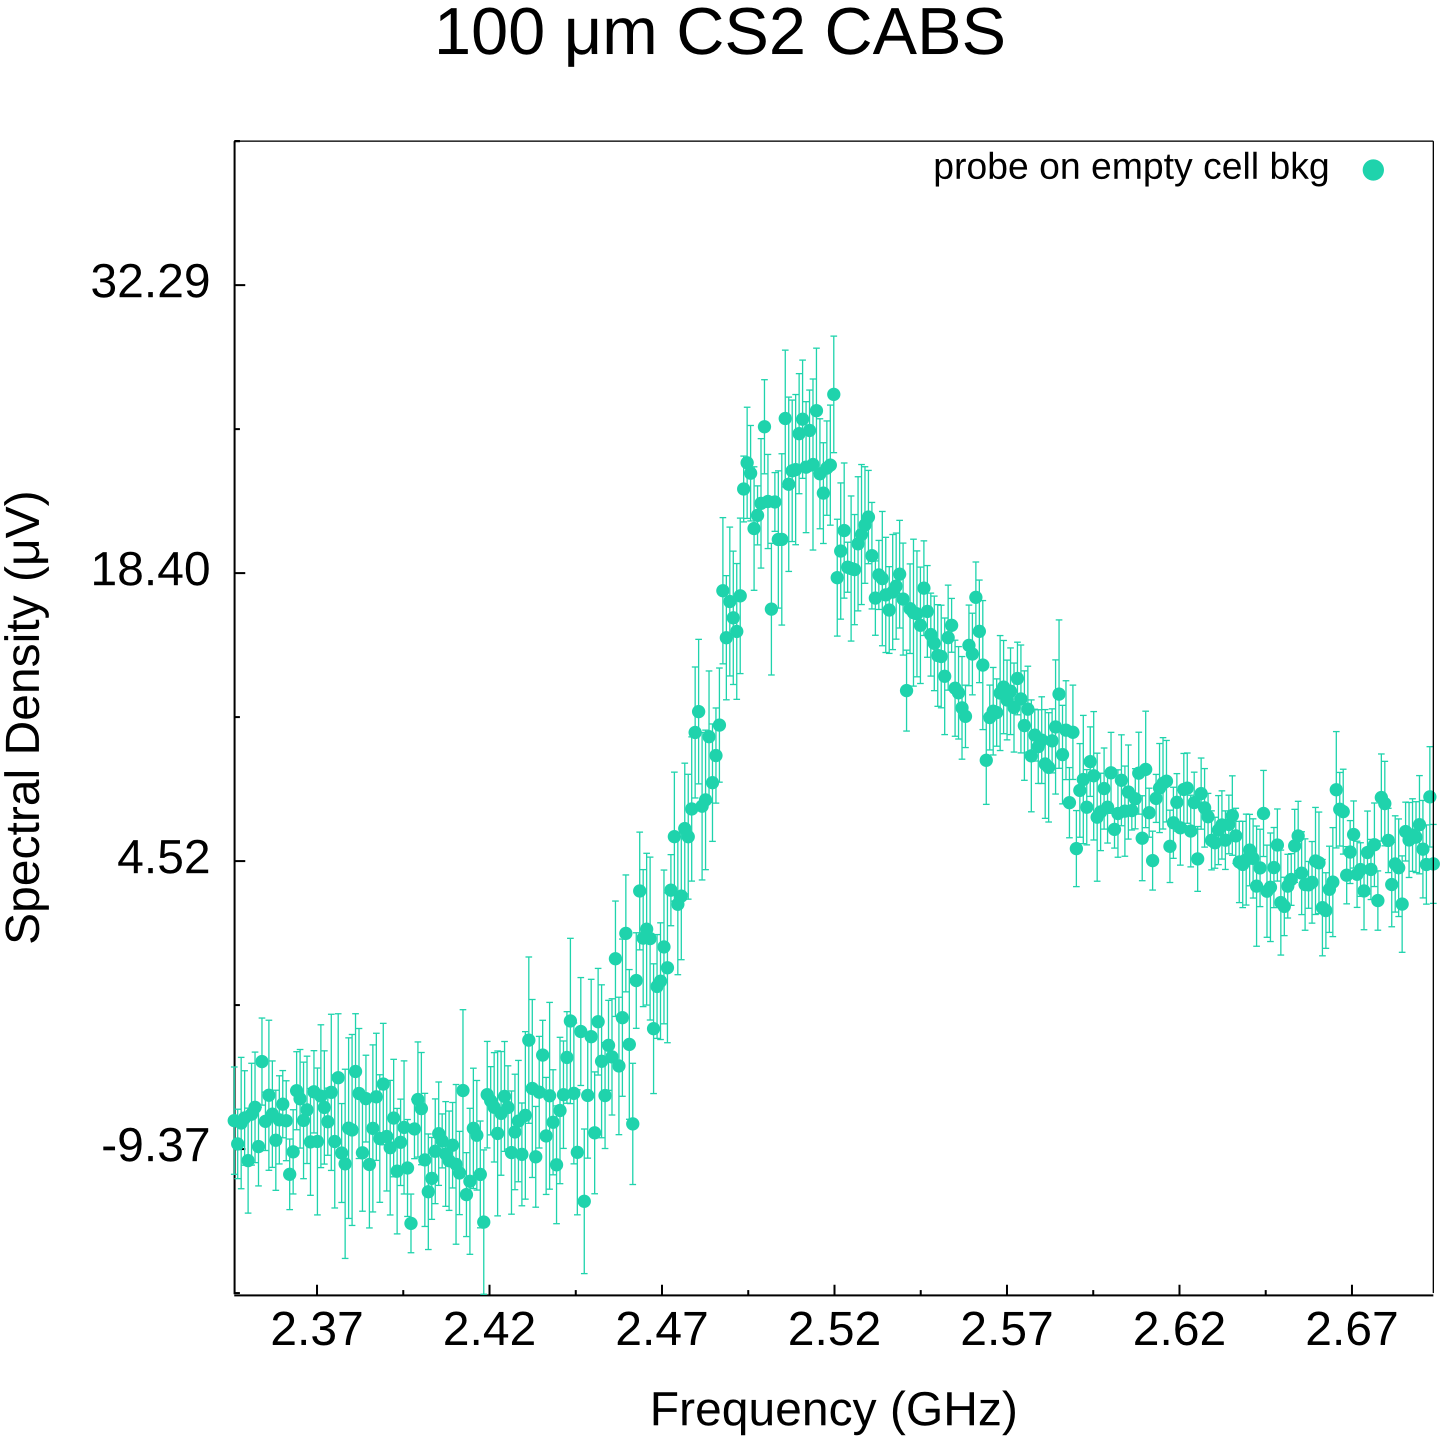
\includegraphics[width=\textwidth]{figs/4-CABS/CABS-100um CS2.png}
        \caption{CABS measurement of 100um of CS2.}
        \label{fig:CABS 100um CS2}
    \end{figure*}

    comparison to stimulated brillouin and spontaneous brillouin?

  \subsection{Phase-Matching in Small L Regime}
  \label{subsec:CABS:Results:Phase-Matching}
  \lipsum[1]
  figure: phase-matching
    peak vs pump-probe separation 1cm uhna3, CS2
    peak vs pump-probe separation 1mm uhna3, CS2

\section{Discussion}
\label{sec:CABS:Discussion}
\lipsum[1]

%The following are the topics I brainstormed out for possible appendices for
%the cabs paper as of 10-29-2024

%\section{Instrument Details}
%\subsection{List of Salient Components}
%\subsection{Laser Output: Whisper Mode vs. Dither Mode}
%\subsection{Lock-in Settings}

%\section{Experimental Techniques}
%\subsection{Background Subtraction: Probe Off, Sample In}
%\subsection{Background Subtraction: Probe On, Sample Out}
%\subsection{Polarization Control Limit}
%\subsection{Pump, Stokes, Probe Polarization Optimization}
%\subsection{Local Oscillator Polarization Optimization}
%\subsection{Lock-in Detector Settings}
%\subsection{Detection Bandwidth}

%\section{Pump, Stokes, and Probe Contribute Equally}

%\section{Comparison to SBS}
%\subsection{1 Centimeter UHNA3 Scattered Power}
%\subsection{100 Micrometers CS2 Scattered Power}

%\section{Measurement Theory}
%\subsection{Heterodyne Detection}
%\subsection{Lock-in Detection}

%\section{Sensitivity}
%\subsection{Sensitivity Measurements}
%\subsection{Current Sensitivity Limitors}
%\subsection{Ultimate Sensitivity Limitor: Shot Noise}

%\section{Alternative Configurations}
%\subsection{Mirrored Design}
%\subsection{Radial Acoustic Modes}
%\subsection{Shear Acoustic Modes}
%\subsection{Torsional Acoustic Modes}
%\subsection{Coherent Raman Spectroscopy}


%%%%%%%%%%%%%%%%%%%%%%%%%%%%%%%%%%%%%%%%%%%%%%%%%%%%%%%%%%%%%%%%%%%%%%%%%%%
% \clearpage
\setcounter{rownumber}{0}
\singlespacing
\chapter{Brillouin-Induced Raman Modes and Device Exploration}
\label{ch:Raman}
\acresetall

\doublespacing

%%%%%%%%%%%%%%%%%%%%%%%%%%%%%%%%%%%%%%%%%%%%%%%%%%%%%%%%%%%%%%%%%%%%

\section{Introduction}
\label{sec:Raman:Introduction}

This chapter explores progress towards the goal of demonstrating Brillouin-induced Raman-like modes at room temperature. We aim to show that acoustic traveling-wave phonons generated by a Brillouin scattering process in a confined medium can organize into discrete standing-wave vibrational modes. This goal represents a convergence of several themes in modern photonics: cavity optomechanics, coherent phonon control, and nonlinear light–matter interactions. Cavity optomechanics has traditionally focused on discrete mechanical resonances such as drumhead membranes or whispering-gallery (\ac{WGM}) microresonators to achieve effects like laser cooling of vibrational modes or phonon lasing. \cite{kippenberg2008cavity, chan2011laser, aspelmeyer2014cavity, vahala2009phonon} In parallel, Brillouin scattering provides a route to manipulate traveling-wave acoustic phonons in extended media, as demonstrated by our Brillouin-based laser cooling in optical fiber (a “cavity-less” system). \cite{johnson2023laser, eggleton2013inducing, bahl2012observation, otterstrom2018optomechanical} The research in this chapter aims to bridge these domains, leveraging traveling-wave Brillouin scattering in a finite-length system so that the phonons become self-confined, resembling the vibrational modes that give rise to Raman scattering.

This investigation is grounded in the broader context of controlling phonons and light at the mesoscale. High-coherence phonons are garnering interest for precision metrology and quantum information, \cite{balram2016coherent, schliesser2014cavity} spurring new strategies for phonon coherent optomechanical interactions. \cite{kippenberg2008cavity, aspelmeyer2014cavity} Earlier chapters of this dissertation advanced this frontier: Chapter 2 demonstrated the laser cooling of propagating acoustic phonons in an optical fiber, extending optomechanical control to continuous media at room temperature, \cite{johnson2023laser} and Chapter 3 introduced a novel Brillouin spectrometer which offers especially high sensitivity for short (\(<\)\SI{1}{\centi\meter}) lengths over traditional \ac{SBS}. Building on such results, the present work tackles the next challenge: inducing standing-wave acoustic modes in a bulk-like sample through Brillouin processes. Achieving this at room temperature would be significant, as to date strong acoustic mode formation has been mostly limited to cryogenic systems where phonon lifetimes are long. \cite{otterstrom2018optomechanical, galliou2013extremely} By pursuing Brillouin-induced modes under ambient conditions, we push toward practical phonon devices and new regimes of light–sound interaction without the strict need for optical cavities. \cite{pant2011chip}

%--------------------------------------------------------------------%

\section{From Traveling-Wave to Raman-Like Standing-Wave Modes}
\label{sec:Raman:FromTraveling-WavetoRaman-LikeStanding-WaveModes}

\subsection{Review of Brillouin and Raman Scattering}
\label{subsec:Raman:ReviewofBrillouinandRamanScattering}

Brillouin scattering and Raman scattering are two related light–matter interactions that involve inelastic scattering of photons by phonons, but they differ in the nature of the phonons involved. In Brillouin scattering, an incident photon exchanges energy and momentum with a long-wavelength acoustic phonon (a propagating sound wave in the medium). In contrast, Raman scattering typically involves optical phonons or molecular vibrations, which are localized oscillations (e.g. bond vibrations within a molecule or internal lattice vibrations) rather than a continuum acoustic wave. In other words, Brillouin scattering is mediated by traveling acoustic waves in a bulk material, whereas Raman scattering probes standing-wave intramolecular or lattice modes. This fundamental difference is reflected in the frequency scales: acoustic phonons have relatively low frequencies (\si{\giga\hertz} or below) and are responsible for the small Stokes/anti-Stokes shifts in Brillouin spectra, whereas optical phonons and molecular vibrations have much higher frequencies (\si{\tera\hertz}) yielding the larger shifts seen in Raman spectra (see Figure~\ref{fig:Introduction:scattering-domains}). \cite{cardona2007light} It is also reflected in momentum conservation conditions: Brillouin scattering requires phase-matching between the optical wave and an acoustic phonon of a particular wavevector, essentially picking out a traveling phonon mode with a definite momentum. Raman scattering, on the other hand, often involves phonons with near-zero wavevector (e.g. zone-center optical modes in crystals or whole-molecule vibrations) due to the selection rule of crystal momentum conservation in perfect lattices. \cite{ferraro2003introductory}

Despite these distinctions, the line between Brillouin and Raman processes can blur in certain situations. If the medium lacks long-range order or the phonon coherence length is short, the usual momentum-selection rules break down. Shuker and Gammon (1970) \cite{shuker1970raman} showed that in amorphous materials, translational symmetry is lost and essentially all vibrational modes can participate in light scattering. In such cases, even low-frequency acoustic-like modes (normally the realm of Brillouin) become “Raman-active.” This insight explained the observation of broad low-frequency Raman scattering (the so-called boson peak) in glasses by attributing it to acoustic vibrations made allowable by disorder. \cite{duval1990vibrational, winterling1975very, nemanich1977low, martin1974model, malinovsky1986nature, buchenau1986low, malinovsky1987investigation, chumakov2011equivalence} Conversely, in a small or confined system, the vibrational modes are discrete rather than forming a continuous acoustic band. In effect, they approach the molecular limit where each normal mode can scatter light akin to a Raman transition. Thus, one can view Brillouin and Raman scattering as two limits of the same fundamental interaction, distinguished by whether the phonons act as continuous waves or as localized normal modes.

Spatial confinement of acoustic waves can convert the Brillouin regime into a Raman-like regime. In an unbounded or large medium, acoustic phonons exist over a continuum of frequencies and wavevectors (a traveling-wave picture). But if the medium is bounded (e.g., a micron-scale particle or a cavity of finite length) the acoustic field must satisfy boundary conditions, leading to a set of allowed eigenmodes. Classic elasticity theory by Lamb (1882) \cite{lamb1881vibrations} provided the first analysis of this: a homogeneous elastic sphere supports only certain quantized vibration modes (classified into spheroidal and torsional families) dictated by the sphere’s finite size and free-surface boundary condition. These quantized vibration modes are true standing-wave modes confined to the sphere. Subsequent work extended Lamb’s theory to include various effects such as surface tension and clamping for small particles, \cite{} but the essential result is that a finite object has discrete acoustic eigenmodes. Experimentally, Duval et al. (1986) \cite{duval1986vibration} performed a notable demonstration by observing very-low-frequency Raman scattering from nanometer-sized microcrystals embedded in glass. The Raman spectra showed distinct peaks whose frequencies scaled inversely with the particle diameter, exactly as expected for Lamb’s vibrational modes in a sphere. Duval identified these peaks as the confined acoustic eigenmodes (“particle vibrational modes”) of the microcrystallites, which had become Raman-active. This exemplified how a Brillouin-like acoustic wave (here, a sphere’s breathing or shear wave) can become Raman-like when spatially confined. When an acoustic phonon is restricted by boundaries, it is no longer a freely propagating wave but rather a normal mode with a discrete frequency, effectively turning a Brillouin interaction into a Raman-style interaction with a set of allowed modes.

Figure~\ref{fig:Raman:BrillouinRamanTransition} offers a conceptual illustration of the transition from a traveling acoustic wave to standing-wave vibrational modes. In a bulk material (left), light scatters from a continuum of acoustic waves (Brillouin scattering), whereas in a confined medium (right), only discrete phonon modes are allowed, producing Raman-like spectral lines. Spatial confinement and acoustic reflections thus shift the scattering from the Brillouin regime toward a Raman-like regime. Contemporary research in cavity optomechanics and related fields has leveraged this wave-to-mode transition as well. For instance, Renninger et al. (2018) \cite{renninger2018bulk} showed that by shaping the geometry of a \si{\centi\meter}-scale crystal, one can support long-lived acoustic standing-waves even in a bulk solid. At low temperature, the phonon coherence length in their system exceeded the system size, and the crystal effectively behaved as a giant “phonon cavity” with high-Q (quality) acoustic modes. \cite{renninger2018bulk, maccabe2020nano} These modes were accessed via Brillouin interactions, blurring the line between traditional Brillouin and Raman: the process was Brillouin in origin (photoelastic coupling to sound waves) but the phonons were in discrete cavity modes like Raman vibrations. These studies underscore that confined acoustic phonons can take on the character of Raman modes.

\begin{figure}[t]
  \centering
  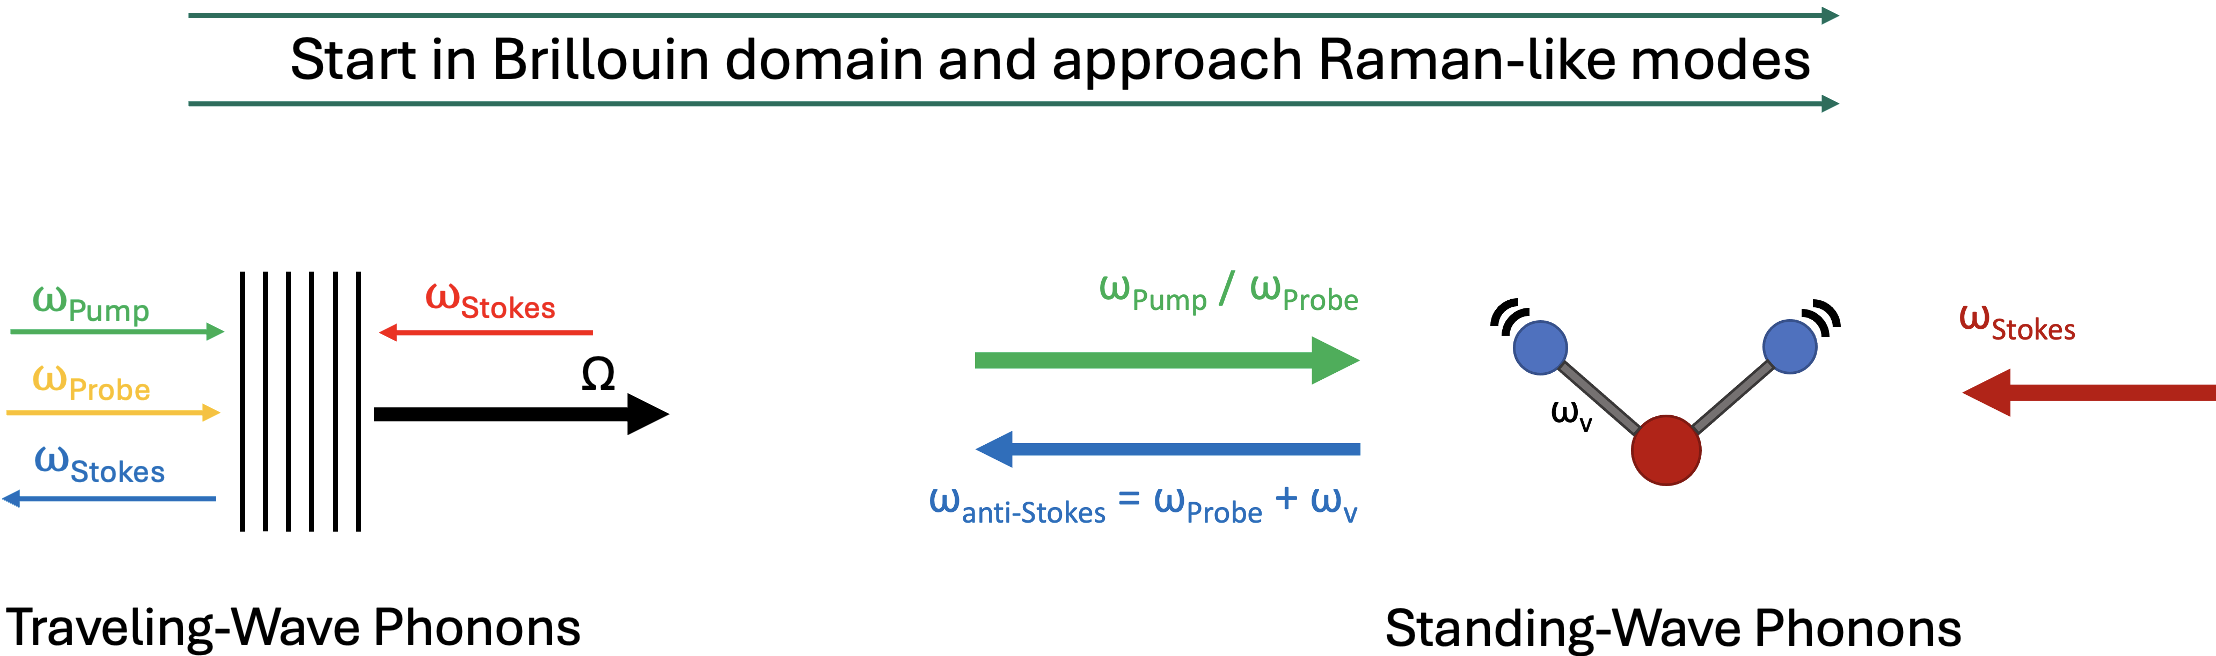
\includegraphics[width=\textwidth]{figs/4-Raman/ExploreBrillouinRamanTransition.png}
  \vspace{0.5em}
  \caption{Conceptual illustration of the transition from a traveling acoustic wave to standing-wave vibrational modes. In a bulk material (left), light scatters from a continuum of (traveling) acoustic waves (Brillouin scattering), whereas in the molecular vibrations of atomic bonds (right), only discrete (standing-wave) phonon modes are allowed. The left diagram is a conceptual visualization of the \ac{CoBS} process for a longitudinally-traveling phonon \(\Omega\) while the right diagram gives a conceptual visualization of an analogous coherently stimulated anti-Stokes Raman scattering process \ac{CARS} with the standing-vibrations \(\omega_{\rm v}\) among bonded atoms in a molecule.}
  \label{fig:Raman:BrillouinRamanTransition}
\end{figure}

\subsection{Brillouin-Induced Raman Modes}
\label{subsec:Raman:Brillouin-InducedRamanModes}

In a traditional SBS experiment, a pump laser drives an acoustic wave through electrostriction, and the scattered Stokes light is down-shifted by the acoustic frequency \(f_{\rm B}\). In an unbounded or long medium, \(f_{\rm B}\) is determined by material properties (sound speed and optical dispersion) and the acoustic wave can be thought of as a traveling grating moving through the medium. If the medium is shortened such that the acoustic wave can reflect off the sample boundaries, the traveling acoustic wave can auto-interfere with itself to form a standing-wave pattern in the medium. Under these system conditions, a phonon induced by \ac{SBS} will propagate to the sample end, reflect (assuming a high acoustic impedance mismatch at the boundary), and traverse the medium in the reverse direction. If the length \(L\) between acoustic interfaces is a half-integer number of acoustic wavelengths, the forward and backward phonon waves can interfere to form a standing wave pattern (i.e., a resonance), in essence trapping the traveling phonon in the cavity defined by the sample. This standing wave in turn acts like a stable grating, enhancing the scattering of light at well-defined frequencies corresponding to its resonances. We term these resonant phonon excitations “Brillouin-induced Raman modes” to reflect their hybrid character.

In more concrete terms, the finite-length system behaves like an acoustic Fabry–Pérot cavity. For a longitudinal acoustic mode, the condition for a standing wave is that an integer number \(n\) of half-wavelengths equals the round-trip length: \(n \cdot (\lambda_{\rm s}/2) = L\). Equivalently, the allowed acoustic frequencies are

\begin{equation}
  f_{\rm n} = \frac{n\,v_{\rm s}}{2L},
  \label{eq:Raman:f_R}
\end{equation}
\\
where \(v_{\rm s}\) is the sound velocity in the medium and \(n = 1, 2, 3, \dots\) indexes the mode order. The lowest-frequency mode (\(n = 1\)) has a fundamental frequency \(f_{\rm 1} \approx v_{\rm s}/(2L)\), and higher modes are integer multiples of this fundamental (assuming a simple one-dimensional confinement). Thus, instead of a single Brillouin shift \(f_{\rm B}\), one expects a ladder of equally spaced phonon modes in the scattering spectrum, resembling a Raman vibrational progression. The spacing \(\Delta f\) between adjacent modes is approximately \(\Delta f \approx v_{\rm s}/(2L)\), set solely by the cavity length and sound speed. Figure~\ref{fig:Raman:GeometryDeterminesFundamentalFreq} illustrates why this is so,  For example, if \(L =\) \SI{10}{\milli\meter} in a medium where \(v_{\rm s} =\) \SI{5000}{\meter\per\second}, the fundamental mode would be \(f_{\rm 1} \sim\) \SI{250}{\kilo\hertz} and overtones at \SI{500}{\kilo\hertz}, \SI{750}{\kilo\hertz}, etc. In principle, a sufficiently short and high-Q acoustic cavity could produce a comb of multiple \si{\giga\hertz}-range lines (analogous to molecular vibrational Raman lines) out of what would ordinarily be a single broad Brillouin gain peak.

\begin{figure}[t]
  \centering
  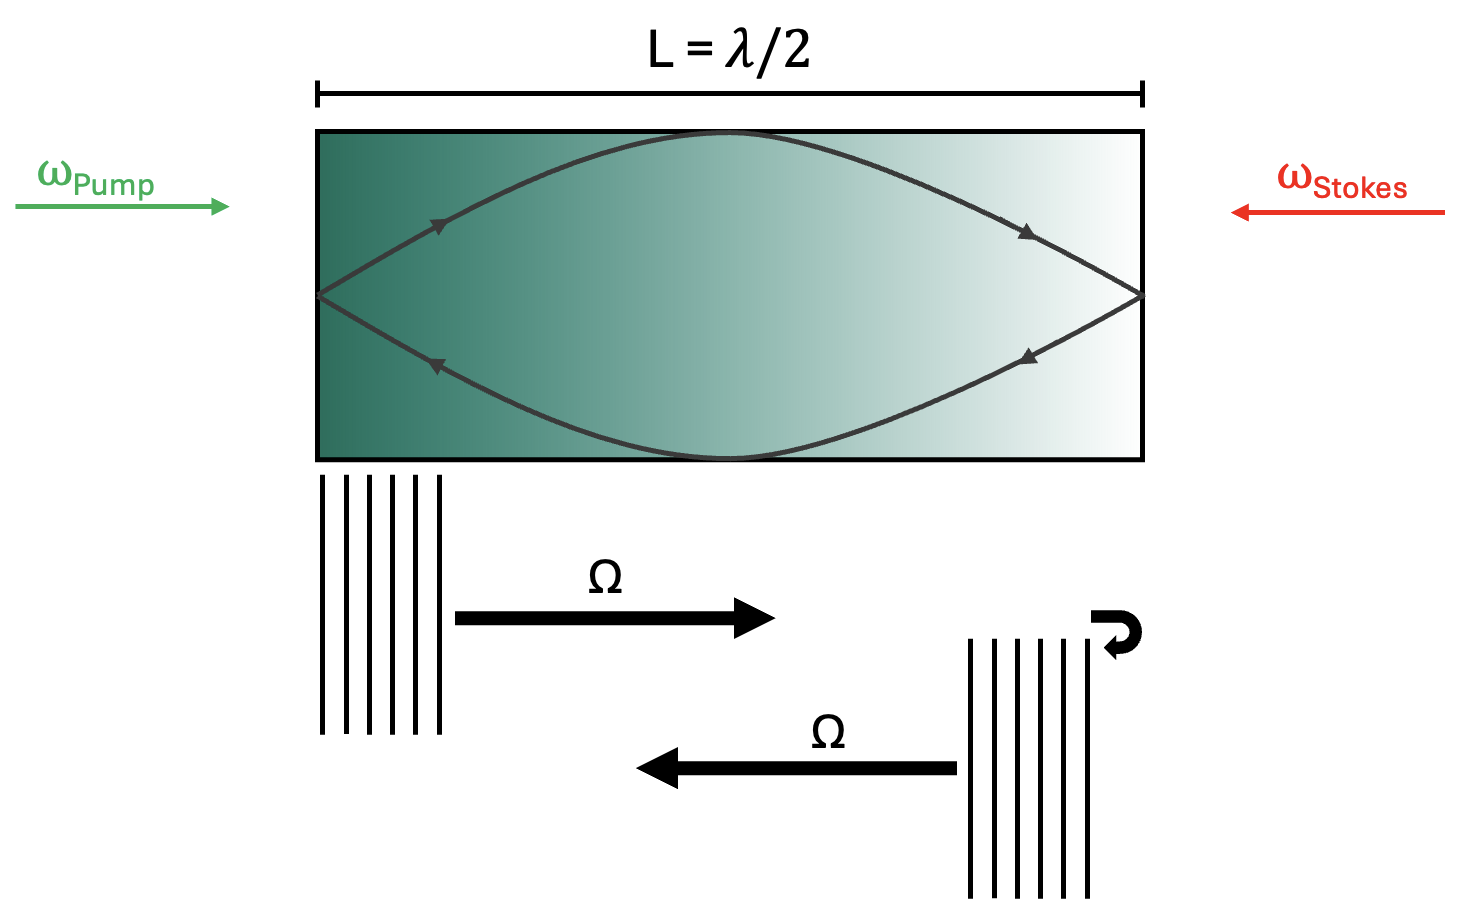
\includegraphics[width=.85\textwidth]{figs/4-Raman/GeometryDeterminesFundamentalFreq.png}
  \caption{Illustration showing how geometry and sound speed of the material determine the allowed acoustic frequencies, given by Equation~\ref{eq:Raman:f_R}. Traveling-wave phonons around the material's Brillouin frequency shift \(f_{\rm B}\) are transduced within the medium via the \ac{CoBS} process. These phonons traverse the length to reach the boundary, where a high acoustic impedance mismatch causes them to reflect at the interface and retraverse the length of the medium in the reverse direction. The spatio-temporal overlap of counterpropagating traveling-wave phonons causes them to interfere, creating an acoustic standing-wave pattern within the material at discrete frequencies determined by the length and sound speed of the material. Shown in the illustration is the half-wavelength fundamental (\(n=1\)) mode, however in general, harmonics near the material's mechanical resonance frequency \(f_{\rm B}\) would be excited in the medium.}
  \label{fig:Raman:GeometryDeterminesFundamentalFreq}
\end{figure}

These Brillouin-induced modes would manifest as distinct peaks in the spectrum of the scattered light. In addition to the usual broadened Brillouin spectrum (with width given by acoustic damping), one would see a series of sharp lines at \(f_{\rm 1}, f_{\rm 2}, f_{\rm 3}, \dots\) around the center scattered frequency. Such a spectrum would be clear evidence that the phonon field is not only a freely propagating wave but also oscillating in discrete standing patterns (i.e., an optically driven acoustic resonator within the material). This is conceptually similar to stimulated Raman scattering in a molecule, where one can get a cascade of Stokes lines corresponding to \(1\hbar\omega_{\rm vib}\), \(2\hbar\omega_{\rm vib}\), \(3\hbar\omega_{\rm vib}\) energy shifts if the pump is intense. Here the “molecular vibration” is replaced by an acoustic cavity mode. If the pump power is high enough to drive the acoustic mode into the nonlinear regime, one might even observe multiple orders of Stokes (and anti-Stokes) as the phonon population builds up in those modes.

The idea of \ac{SBS}-driven acoustic modes has parallels in prior work. In the cryogenic experiment of Renninger et al. mentioned earlier, \cite{renninger2018bulk} a bulk acoustic mode was driven via Brillouin scattering in a \si{\centi\meter}-scale quartz crystal. At low temperatures, they observed ultra-narrow acoustic resonances (indicative of discrete modes) in place of a broad Brillouin response, confirming that acoustic coherence across the entire sample can indeed produce a modal spectrum. In our case, we seek to do this at room temperature by engineering a shorter effective acoustic cavity. We aim to accomplish this by taking advantage of our Coherently Stimulated Brillouin Spectrometer (\ac{CoBS}), which offers \(\sim10^{6}\) improvement in scattered power for \(\sim\)\si{\centi\meter} lengths over traditional \ac{SBS} (see Appendix~\ref{appendix:comparison} for a comparison of scattered power across Brillouin techniques, and specifically Figure~\ref{fig:SponBSvsStimBSvsCoBS} for a comparison by effective length \(L\)).

\subsection{Key Parameters and Feasibility}
\label{subsec:Raman:KeyParametersandFeasibility}

Observing Raman-like standing-wave modes via \ac{SBS} hinges on several key parameters of the system. We identify three especially critical factors: (1) the scattered power, determined by the effective material Brillouin gain and length as well as the optical powers; (2) the acoustic dissipation in the medium, which limits the mean phonon travel distance; and (3) the acoustic boundary reflectivity, determined by impedance mismatch at interfaces, which enables the phonons to reflect and form standing-waves. These parameters together determine whether the phonon will remain a distributed traveling excitation or collapse (blur) into discrete modes. Chapter~\ref{ch:CoBS} describes the \ac{CoBS} instrument, showing that the scattered power as a result of the \ac{CoBS} process is given by Equation~\ref{Eq:Theoretical Framework:Scattered Power}, stated here again as

\begin{equation}
  P_{\rm Signal} = \frac{1}{4}(G_{\rm B}L)^{2}P_{\rm Pump}P_{\rm Stokes}P_{\rm Probe}\Phi,
  \label{eq:Raman:ScatteredPowerPhi}
\end{equation}
\\
where \(G_{\rm B}\) is the material-dependent effective (acousto-optic overlap-adjusted) Brillouin gain factor given by Equation~\ref{Eq:Effective Brillouin Gain}, \(L\) is the effective length, \(P_{\rm i}\) are the optical powers of the pump, Stokes, and probe waves, respectively, and \(0 < \Phi < 1\) is a phase-matching relaxation term (given by Equation~\ref{Eq:Phi}) that captures the pump-probe detuning on which the instrument relies. A material’s Brillouin gain coefficient \(g_{\rm 0}\) (\si{\watt\per\meter}), or overlap‐adjusted effective gain \(G_{\rm B}\) (\si{\per\watt\per\meter}), sets how strongly the phonons are driven for given pump \(P_{\rm P}\), Stokes \(P_{\rm S}\), and probe \(P_{\rm Pr}\) optical powers over an interaction length \(L\) in the \ac{CoBS} process (see Chapter~\ref{ch:CoBS}, and specifically Equation~\ref{Eq:Theoretical Framework:Scattered Power}), given here again by

\begin{equation}
  G_{\rm B} = \frac{g_{0}}{A_{\rm eff}}\frac{\left(\frac{\Gamma_{\rm B}}{2}\right)^{2}}{\left(\Omega - \Omega_{\rm B}\right)^{2} + \left(\frac{\Gamma_{\rm B}}{2}\right)^{2}}.
  \label{eq:Raman:GB}
\end{equation}
\\
Here, \(\Gamma_{\rm B}\) is the angular Brillouin linewidth, \(\Omega\) (\(\Omega_{\rm B}\)) is the (resonant) angular acoustic frequency, \(A_{\rm eff}\) is the effective area (acousto-optic mode overlap), and \(g_{0}\) is the Brillouin gain coefficient given by

\begin{equation}
  g_{0} = \frac{\gamma_{\rm e}^{2}\omega^{2}}{nv_{\rm s}c^{3}\rho_{0}\Gamma_{\rm B}},
  \label{eq:Raman:g0}
\end{equation}
\\
where \(\gamma_{\rm e}\) is the electrostrictive constant, \(\omega\) is the angular optical frequency, \(n\) is the refractive index, \(v_{\rm s}\) is the speed of sound in the material, \(c\) is the speed of light, and \(\rho_{0}\) is the mean density of the material. Short samples demand very high effective Brillouin gain to achieve significant scattered power in a small \(L\). Certain tellurium‐based materials, for instance, can offer gains orders of magnitude higher than silica, \cite{sanghera2010nonlinear, abedin2005observation} allowing measureable scattered power in sub‐\si{\milli\meter} cavities.

Even if phonons are driven strongly, they must live long enough (i.e., have a low enough dissipation rate, or high enough acoustic Q) to form a standing wave. At room temperature, intrinsic damping can limit phonon \(Q_{\rm s}\) to \(\sim10^{3}\)–\(10^{4}\) in many solids, \cite{heiman1979brillouin, bucaro1974high} implying attenuation lengths of \si{\milli\meter} to \si{\centi\meter} for \si{\giga\hertz} frequencies. Ideally, the sample length \(L\) should be comparable to or less than half the attenuation length so that phonons undergo multiple round trips. This is considerably more difficult at room temperature than at cryogenic temperatures, where \(Q_{\rm s}\) can exceed \(10^{7}\). \cite{maris1990phonon, renninger2018bulk} Finally, the phonon must reflect rather than escape at the boundaries. A large acoustic impedance mismatch (e.g., a free surface with air on one side) can approach nearly 100\% reflection. \cite{galliou2013extremely, auld1973acoustic} Designing the sample with two opposing highly acoustically reflective boundaries is essential to generating a Raman-like standing-wave mode in the medium. In practice, however, partial reflections at each (or even just one) end can suffice so long as the net round‐trip reflectivity is high enough to sustain a mode.

In short, we want to create a high-\(Q\) acoustic resonator inside a Brillouin-active medium at room temperature: strong enough acousto-optic driving to excite the phonons, low enough damping to maintain them, and robust boundary reflections to confine them. Meeting all of these conditions can be challenging. However, the high (\(\sim\)\SI{5}{\femto\watt}) sensitivity and unique short path length advantage of our \ac{CoBS} instrument (described in Chapter~\ref{ch:CoBS} and Section~\ref{appendix:comparison}) sparks new motivation, as it provides a new technique tailored for observing small-scale scattering phenomenon. Feasibility estimates and initial \ac{CoBS} measurements indicate that by utilizing ultra-high-gain media such as \ce{Te} \cite{sanghera2010nonlinear, abedin2005observation} or liquid \ce{CS2} \cite{boyd2020nonlinear}, and ensuring at least one boundary is acoustically reflective, one can push toward Brillouin-induced Raman modes even under ambient conditions.

The sensitivity of our instrument, representing the minimum scattered power that may be detected, has been measured at \(P_{\rm Signal}\approx\) \SI{5}{\femto\watt} (see Section~\ref{Results:Instrument sensitivity}, and specifically Table~\ref{tab:CoBS:5fWSensitivity} together with Equation~\ref{Eq:Theoretical Framework:Scattered Power} and Figure~\ref{fig:CoBS:5fWSensitivity} for validation of this claim). Using this sensitivity value for \(P_{\rm Signal}\) we can rearrange Equation~\ref{eq:Raman:ScatteredPowerPhi} to solve for the minimum length \(L\) we can expect to observe scattering within for given optical powers, material gain, and pump-probe detuning:

\begin{equation}
  L = \frac{2}{G_{\rm B}}\sqrt{\frac{P_{\rm Signal}}{P_{\rm Pump}P_{\rm Stokes}P_{\rm Probe}\Phi}},
  \label{eq:Raman:minimumL}
\end{equation}
\\
where \(0 < \Phi < 1\) and increases for smaller \(L\). For \(P_{\rm Signal}\approx\)\SI{5}{\femto\watt} sensitivity and maximum optical powers \(P_{\rm Pump}P_{\rm Stokes}P_{\rm Probe}=\) \SI{0.25}{\cubic\watt} under typical conditions, Equation~\ref{eq:Raman:minimumL} predicts, for example, the ability to observe scattering within \(\sim\)\SI{500}{\nano\meter} of \ac{UHNA3} fiber (\(G_{\rm B,\,UHNA3}=\) \SI{0.6}{\per\watt\per\meter}). Equation~\ref{eq:Raman:minimumL} makes clear that minimizing the observable scattering length is accomplished by any of: bumping optical powers, improving instrument sensitivity, or choosing a higher gain scattering medium.

In what follows, we detail the experimental platforms and theoretical modeling that guided our attempts to observe discrete phonon modes in high-gain materials. Although a conclusive demonstration proved elusive, the conceptual framework is robust and provides a foundation for ongoing efforts. By shrinking the acoustic path length, maximizing phonon reflectivity, and exploiting strong \ac{CoBS} gain, one can approach the regime where traveling-wave Brillouin scattering morphs into Raman-like standing-wave modes. This pursuit effectively unifies the traveling-wave and standing-wave paradigms of light-sound interaction, providing new opportunities in cavity-free phononics, resonant optomechanics, and coherent phonon devices at room temperature.

\begin{figure}[t]
  \centering
  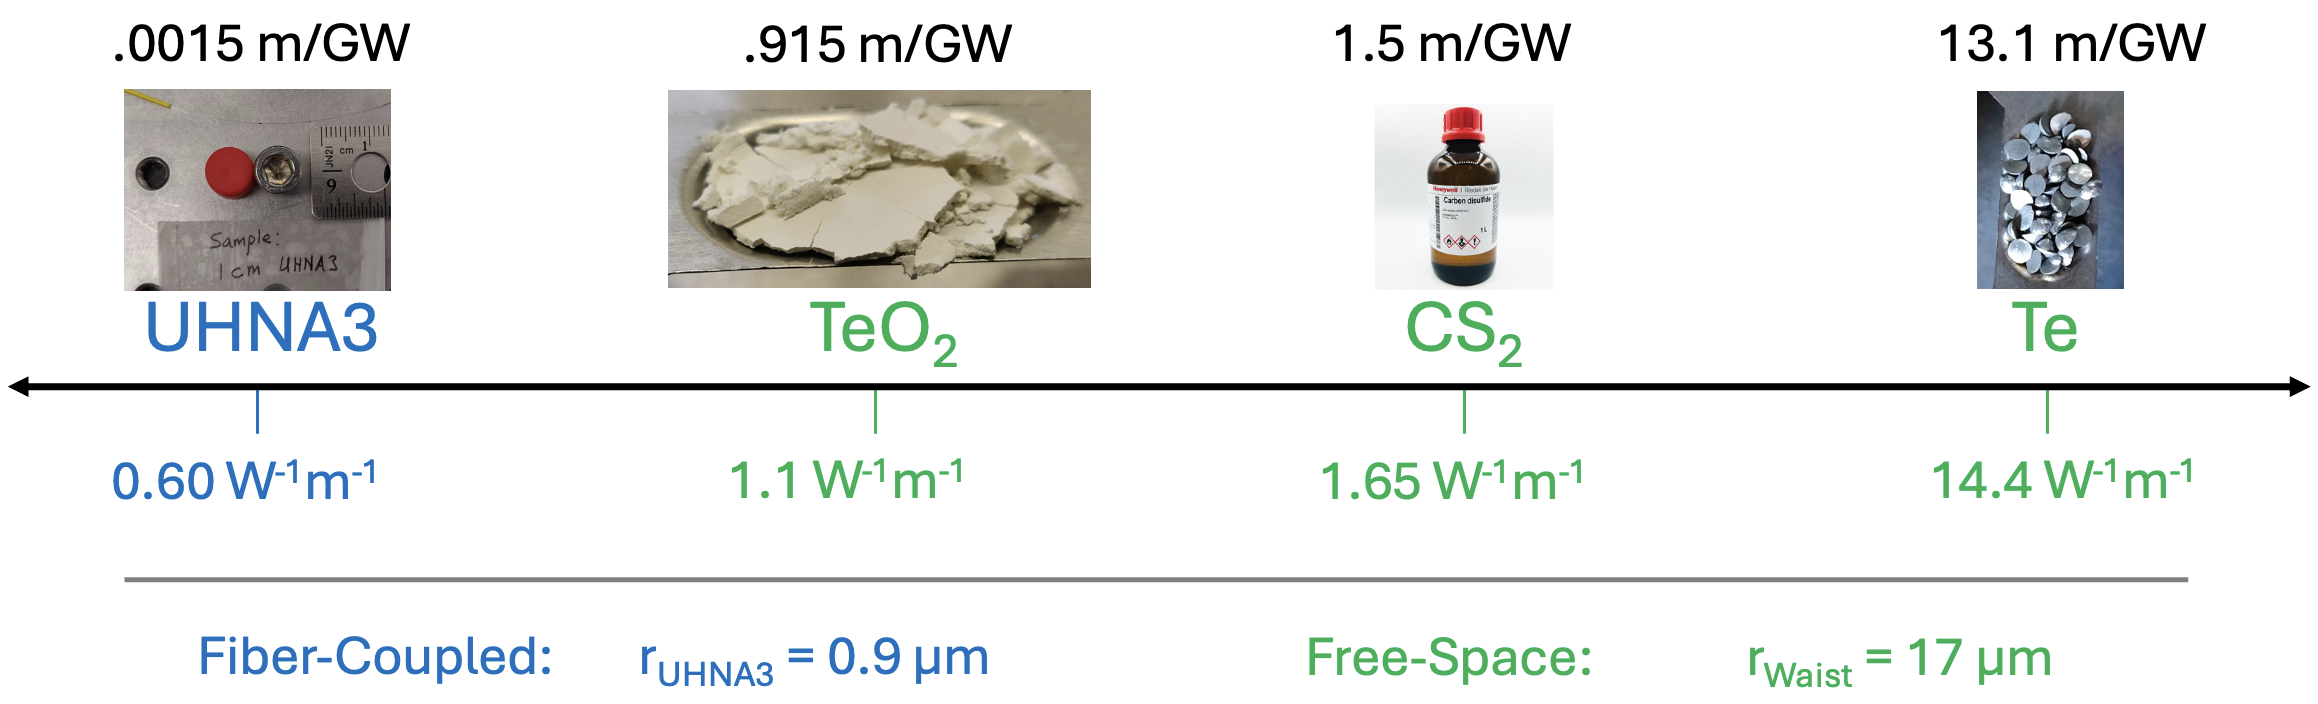
\includegraphics[width=\textwidth]{figs/4-Raman/GainOfRelevantMaterials.png}
  \caption{Gain of relevant materials.}
  \label{fig:Raman:GainOfRelevantMaterials}
\end{figure}

%--------------------------------------------------------------------%

\section{Results}
\label{sec:Raman:Results}

Plots
\begin{itemize}
  \item UHNA3 - 1cm, 1mm
  \item CS2 vial - 4mm, 2mm
  \item TeO2 films - 1um, 500nm
  \item CS2 - 1mm, 100um, (10um not quite)
  \item chip waveguide - chip/nochip, holes
\end{itemize}

\subsection{Germanium-Doped Optical Fiber}
\label{subsec:Raman:Target:UHNA3}

\begin{itemize}
  \item 1cm, 1mm
\end{itemize}

\begin{figure}[t]
    \centering
    \begin{subfigure}[b]{0.49\textwidth}
        \centering
        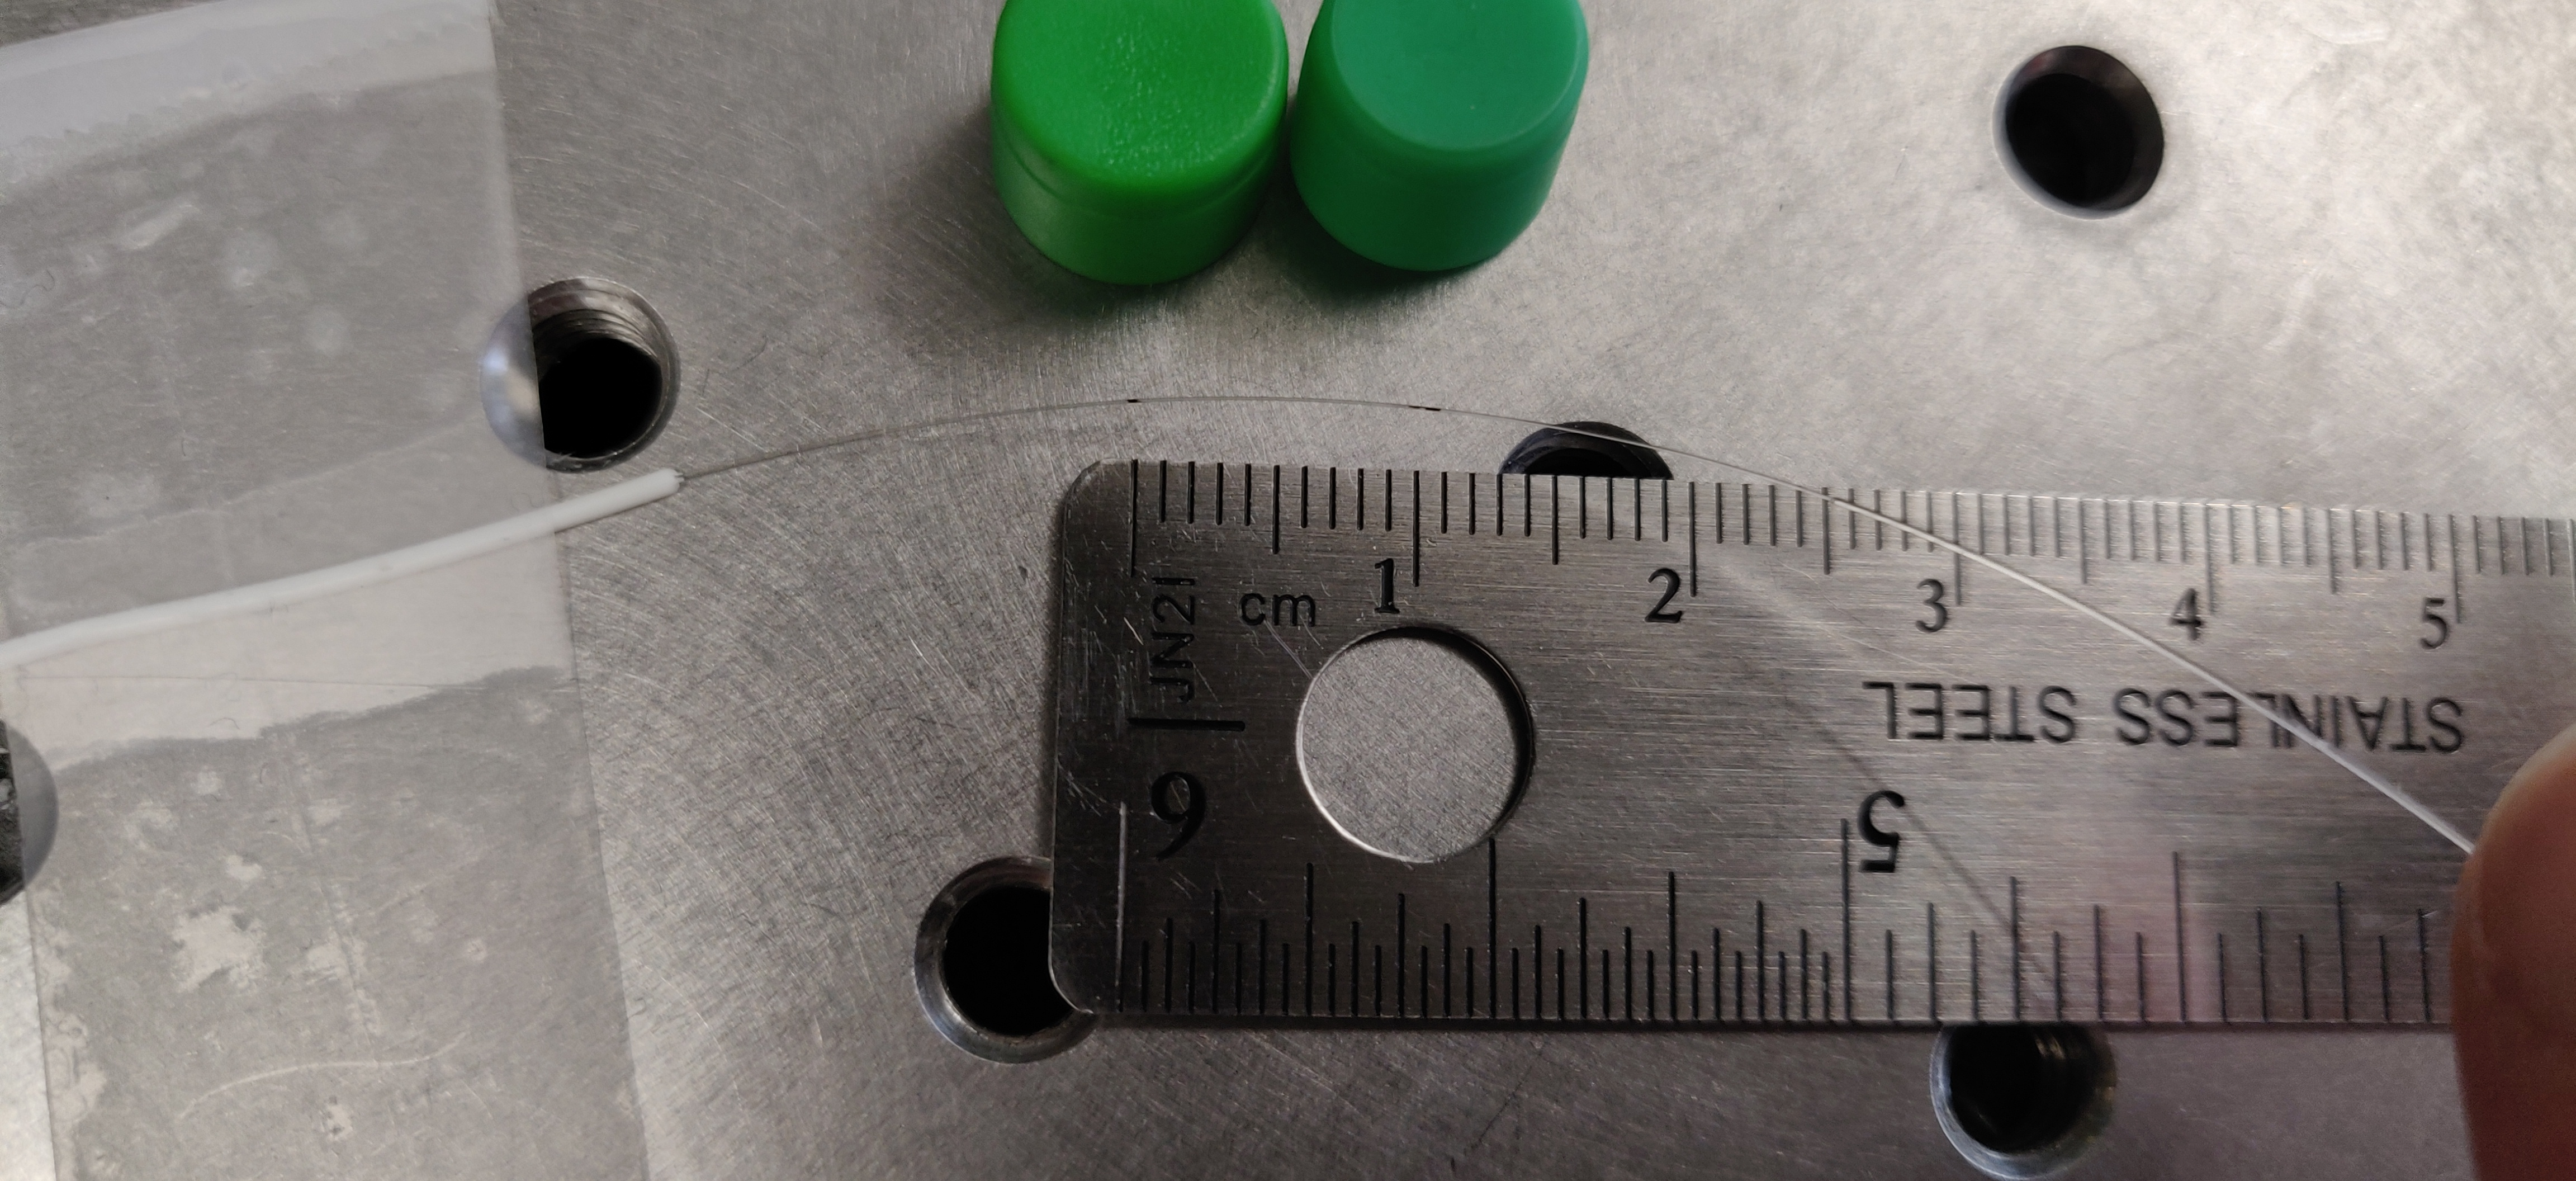
\includegraphics[width=\textwidth]{figs/4-Raman/1cm UHNA3.jpeg}
        \caption{}
        \label{fig:Raman:1cmUHNA3pic}
    \end{subfigure}
    \hfill
    \begin{subfigure}[b]{0.49\textwidth}
        \centering
        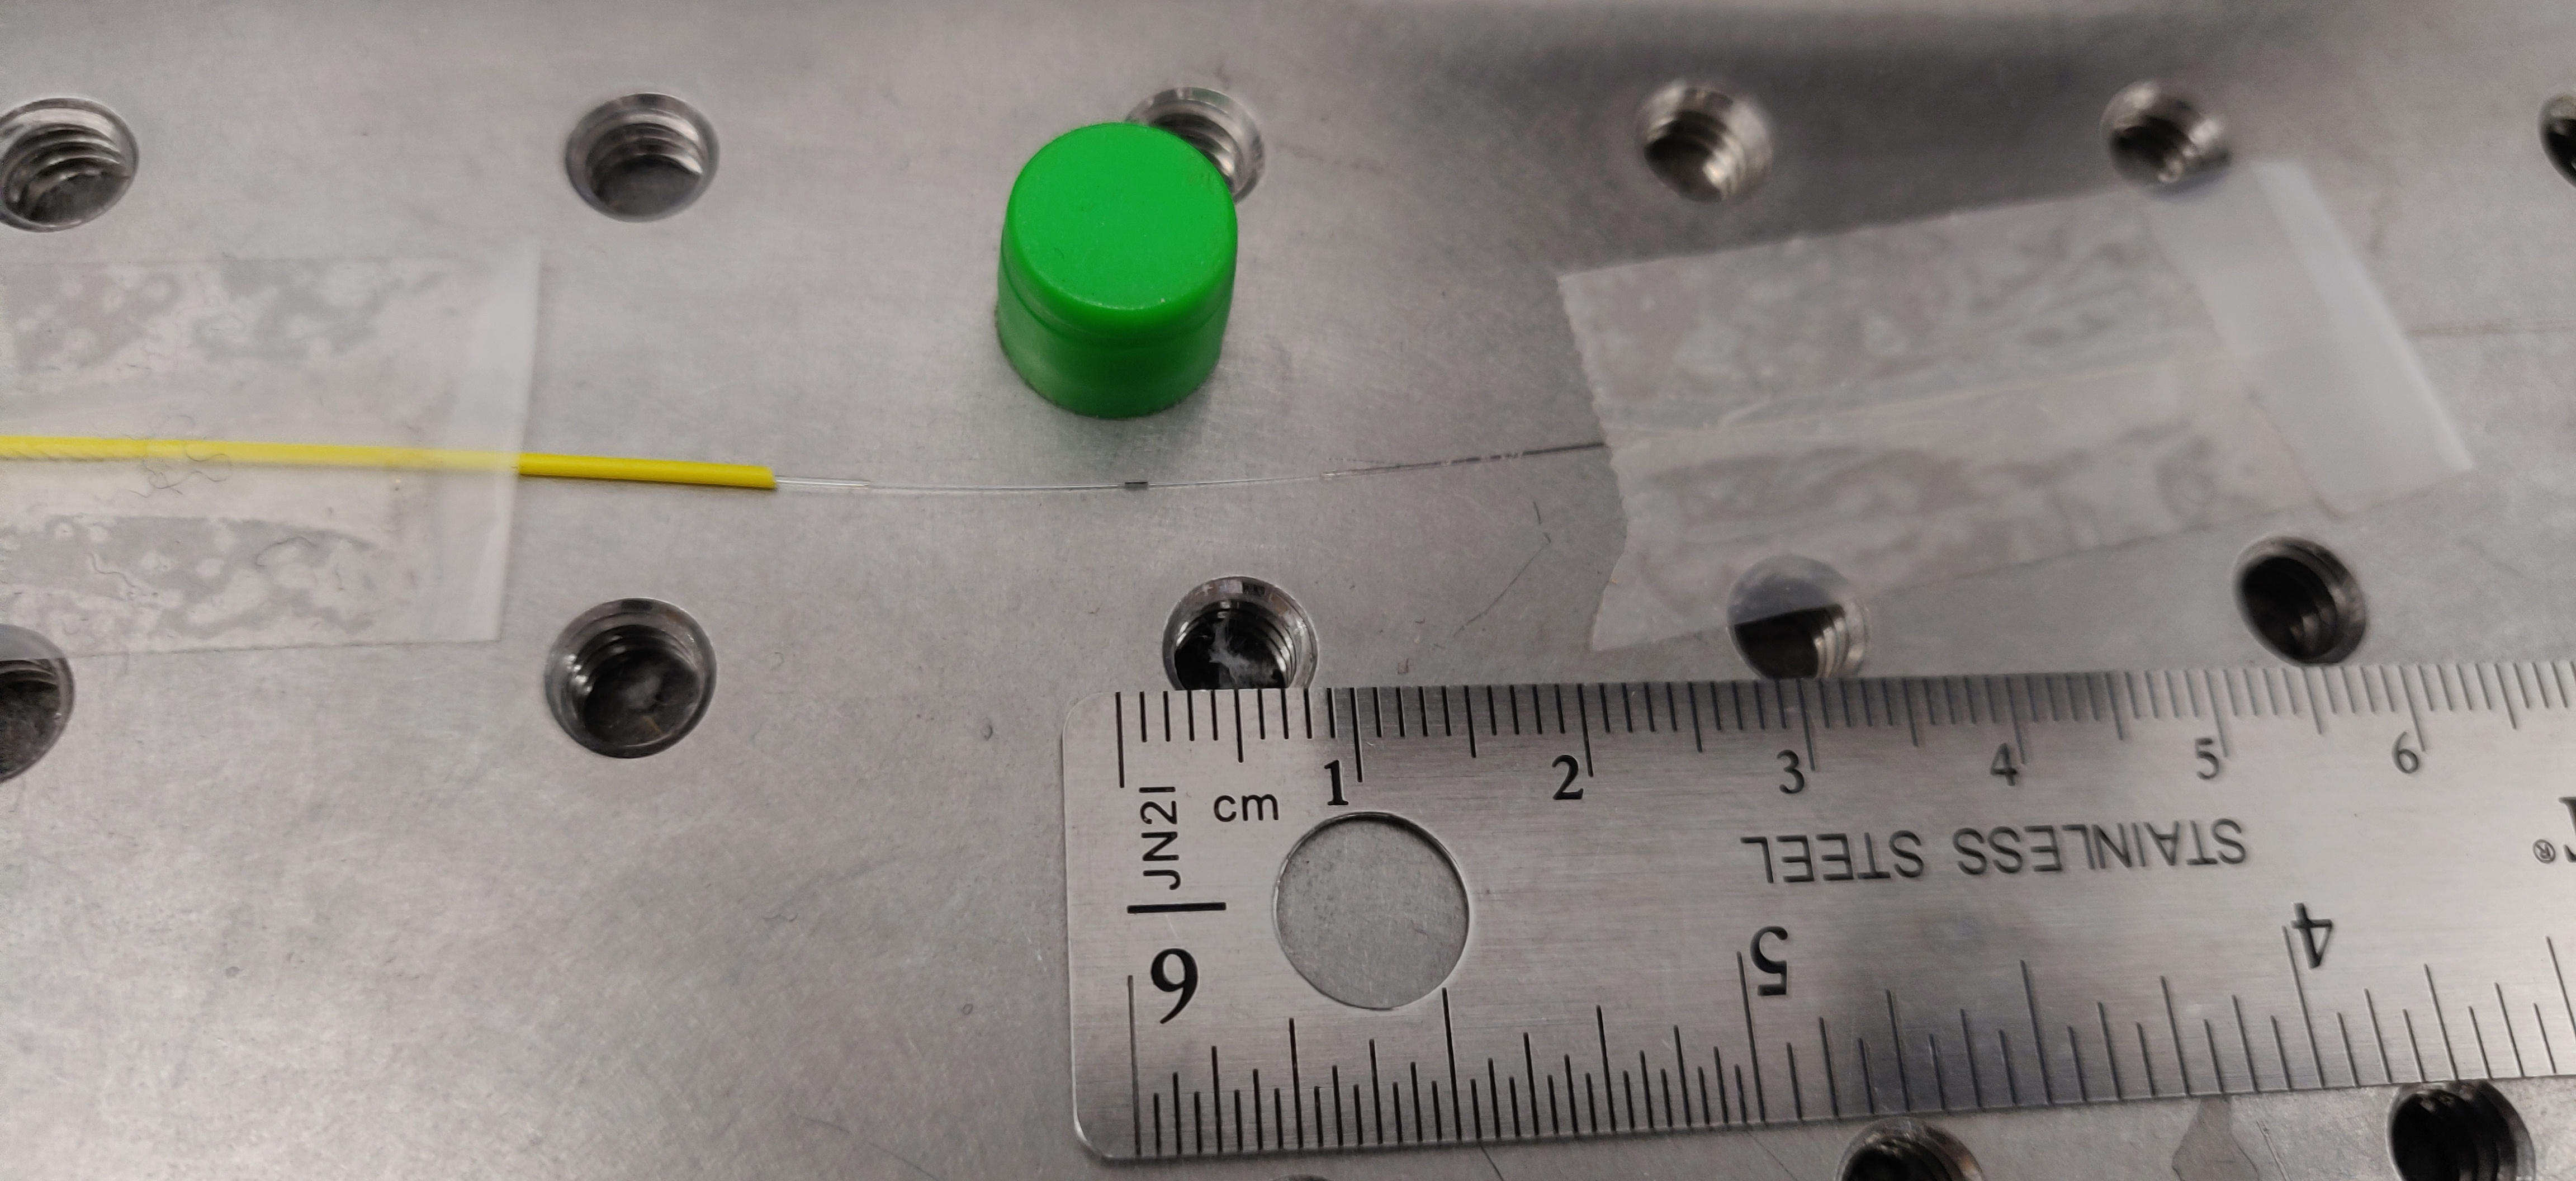
\includegraphics[width=\textwidth]{figs/4-Raman/1mm UHNA3 in apparatus.jpeg}
        \caption{}
        \label{fig:Raman:1mmUHNA3pic}
    \end{subfigure}
    \caption{\SI{1}{\centi\meter} (\ref{fig:Raman:1cmUHNA3pic}) and \SI{1}{\milli\meter} (\ref{fig:Raman:1mmUHNA3pic}) \ac{UHNA3}.}
    \label{fig:Raman:UHNA3}
\end{figure}

\subsection{Free-Space Optics with Liquid Carbon Disulfide}
\label{subsec:Raman:Target:CS2Vial}

\begin{itemize}
  \item Free space with vial
\end{itemize}

\begin{figure}[t]
    \centering
    \begin{subfigure}[b]{0.49\textwidth}
        \centering
        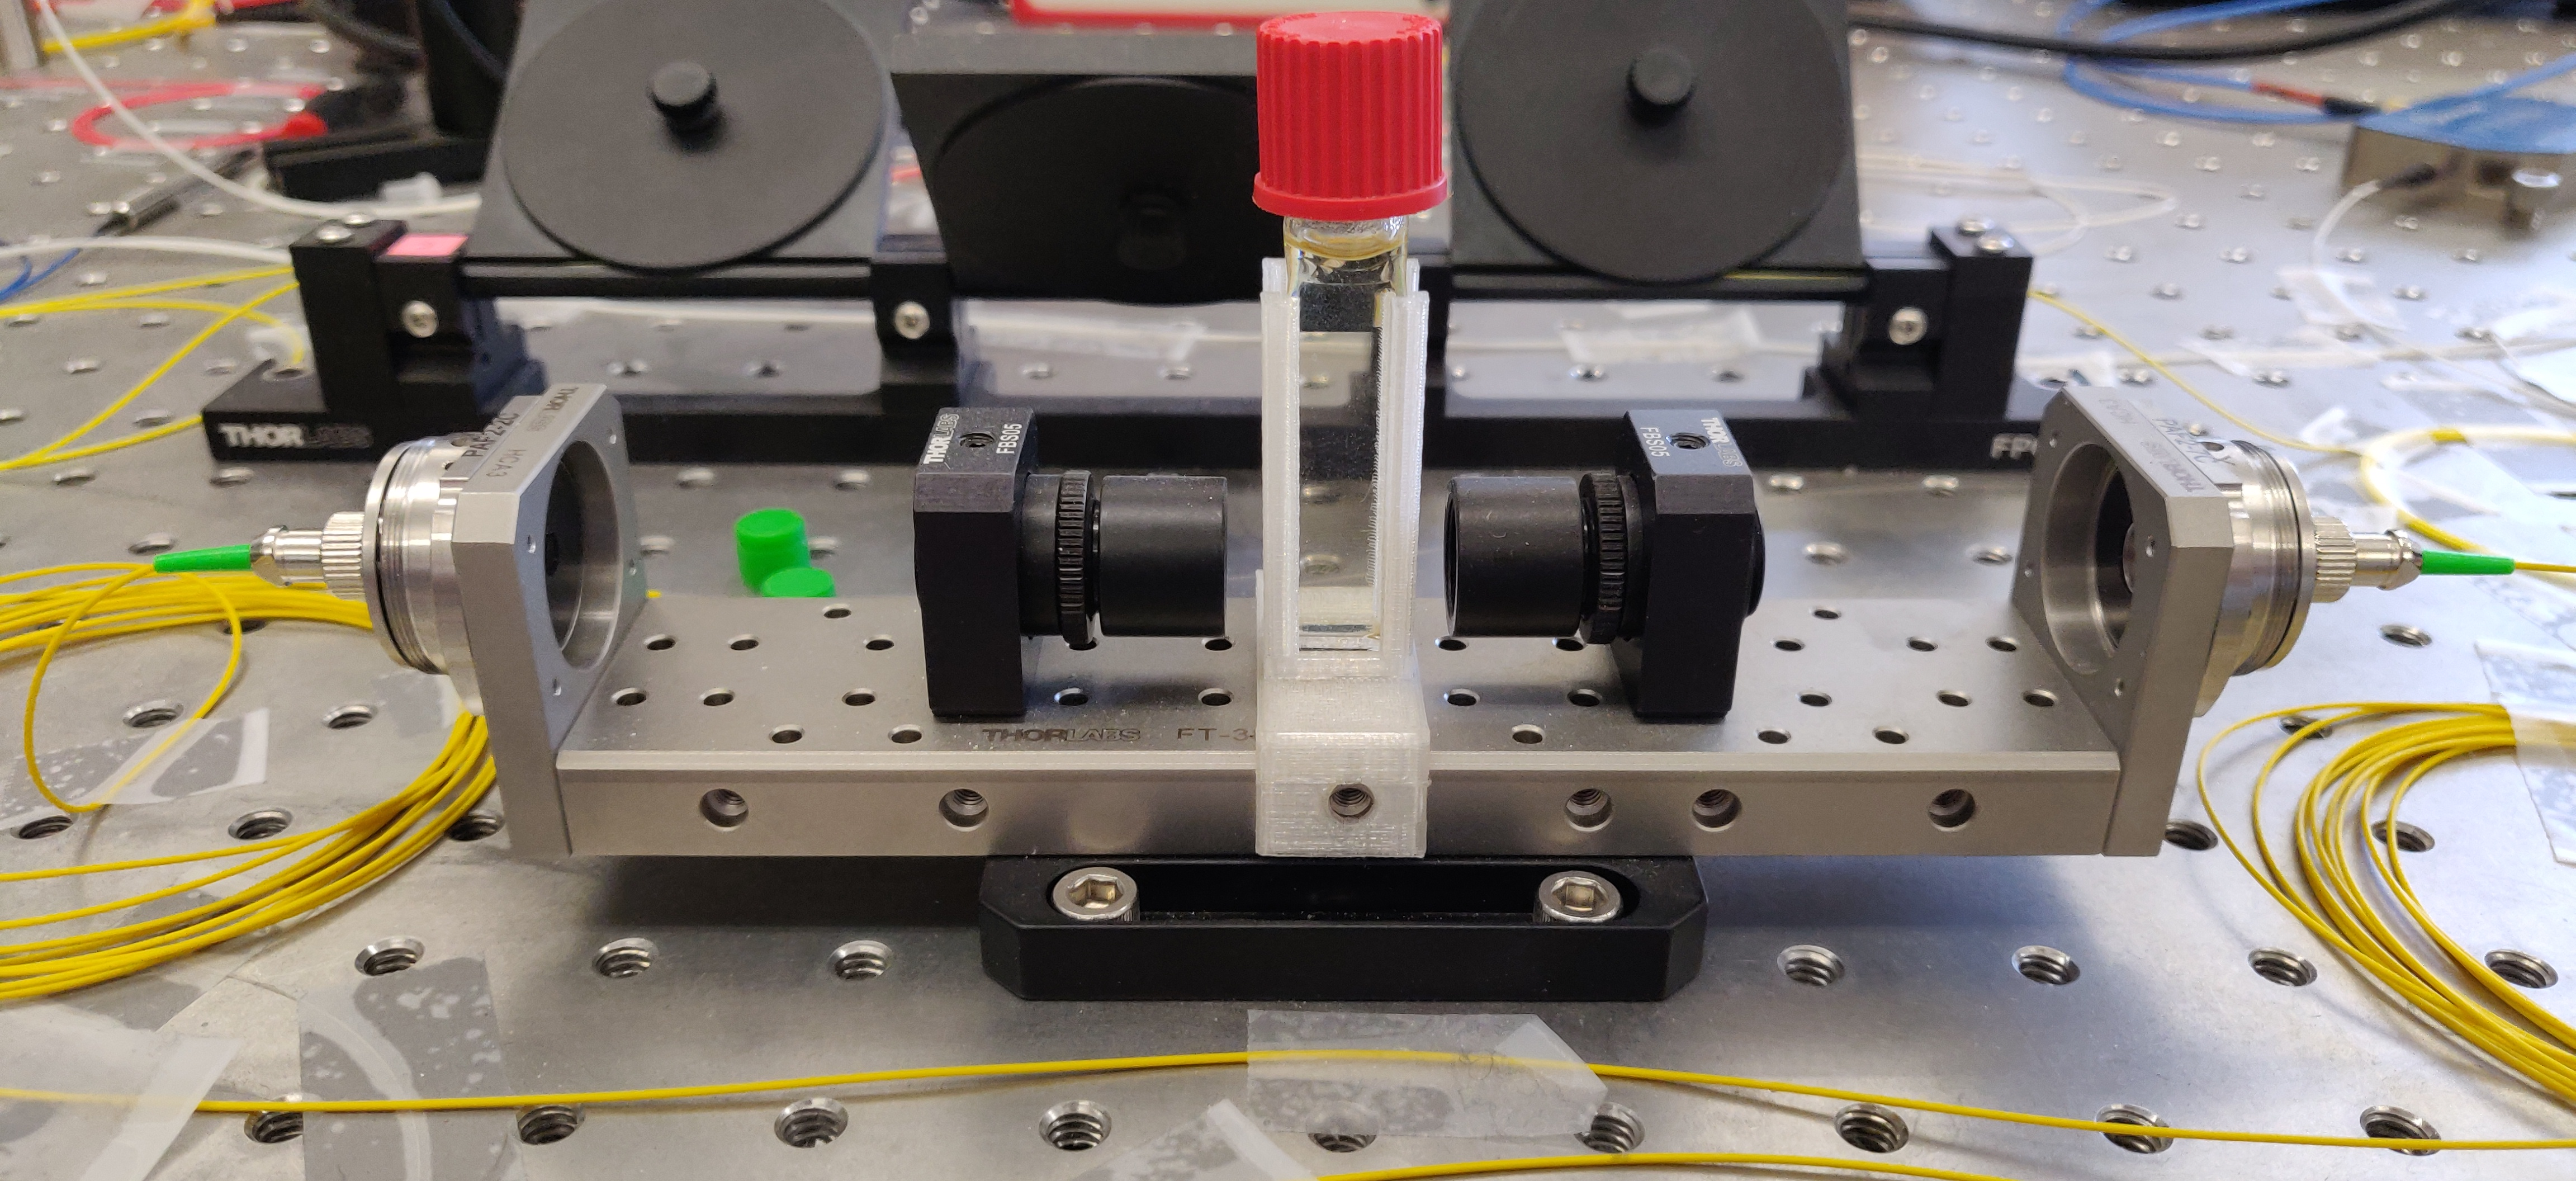
\includegraphics[width=\textwidth]{figs/4-Raman/1cmCS2.jpeg}
        \caption{}
        \label{fig:Raman:1cmCS2}
    \end{subfigure}
    \hfill
    \begin{subfigure}[b]{0.49\textwidth}
        \centering
        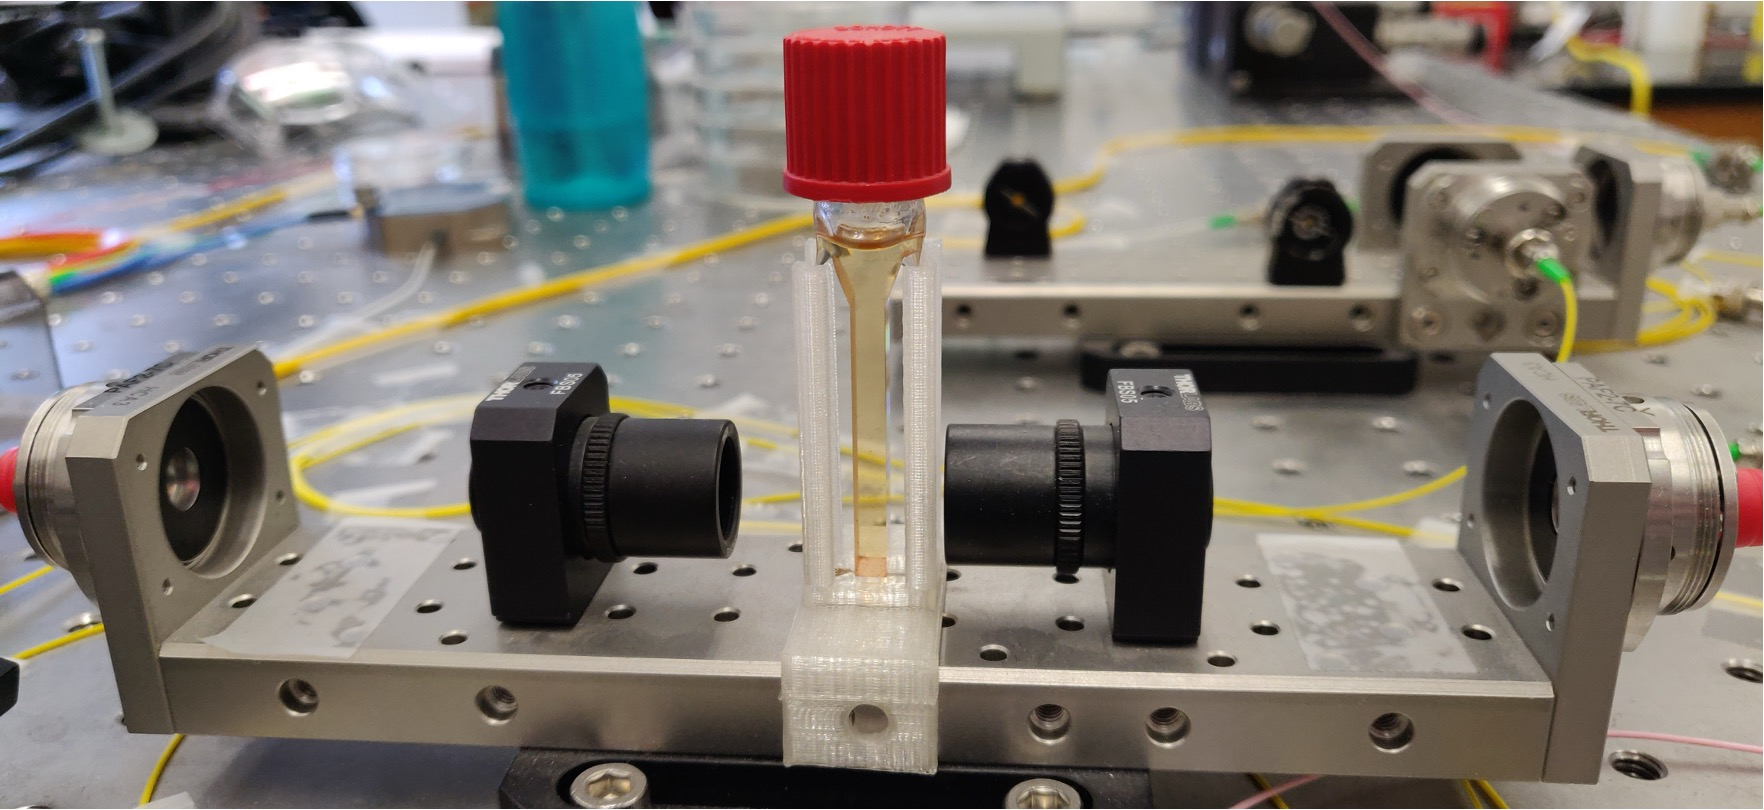
\includegraphics[width=\textwidth]{figs/4-Raman/4mmCS2.jpg}
        \caption{}
        \label{fig:Raman:4mmCS2}
    \end{subfigure}
    \caption{\SI{1}{\centi\meter} (\ref{fig:Raman:1cmCS2}) and \SI{4}{\milli\meter} (\ref{fig:Raman:4mmCS2}) liquid \ce{CS2}.}
    \label{fig:Raman:CS2Cuvet}
\end{figure}

\subsection{Tellurium Dioxide Thin Film}
\label{subsec:Raman:Target:TeO2}

\begin{itemize}
  \item Gibbs collab
  \item deposit Te, oxidize into TeO2
  \item table of relevant TeO2 parameters
\end{itemize}

\subsection{Tellurium Thin Film}
\label{subsec:Raman:Target:Te}

\begin{itemize}
  \item Gibbs collab and CINT collab
  \item oxidizes to TeO2
  \item table of relevant Te parameters
\end{itemize}

\begin{figure}[t]
  \centering
  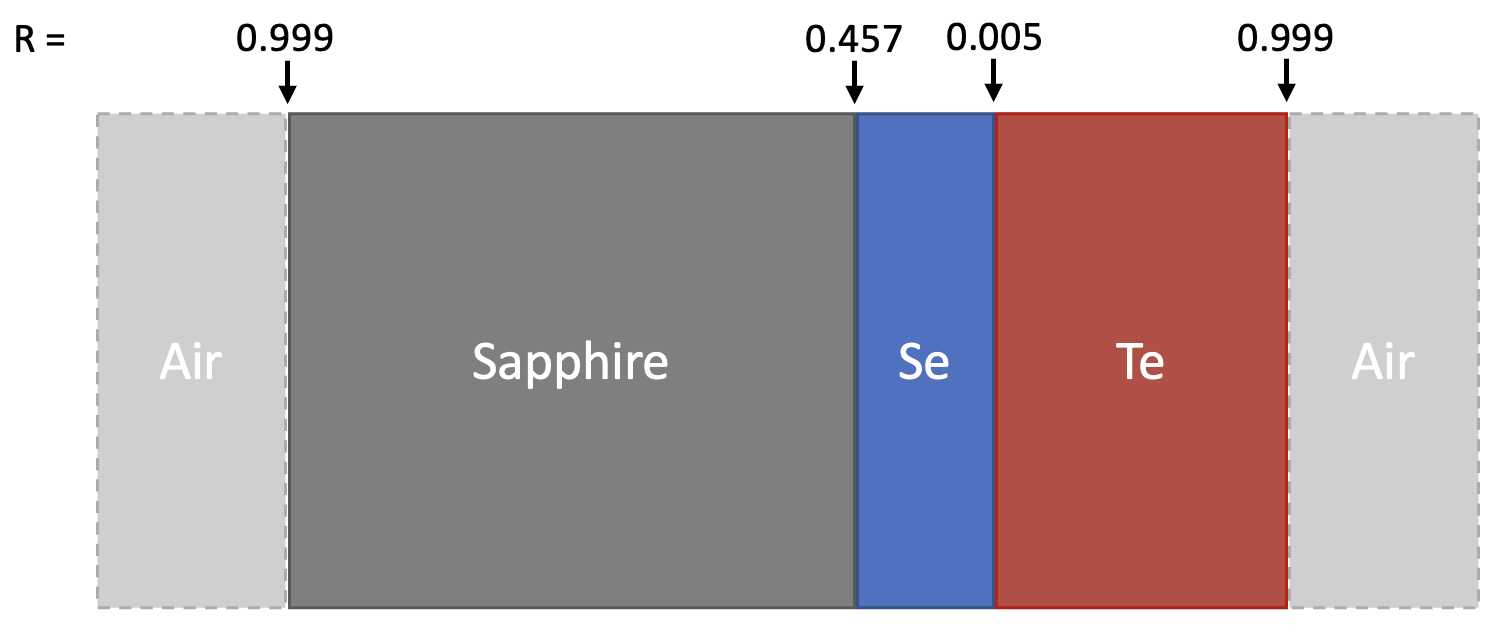
\includegraphics[width=.8\textwidth]{figs/4-Raman/AcousticImpedance.png}
  \caption{Acoustic impedance.}
  \label{fig:Raman:AcousticImpedance}
\end{figure}

\subsection{Carbon Disulfide Micrometer Cell}
\label{subsec:Raman:Target:CS2Cells}

\begin{itemize}
  \item table of relevant CS2 parameters
  \item cells, 1 W amp, bubble test
\end{itemize}

\begin{figure}[t]
    \centering
    \begin{subfigure}[b]{0.3\textwidth}
        \centering
        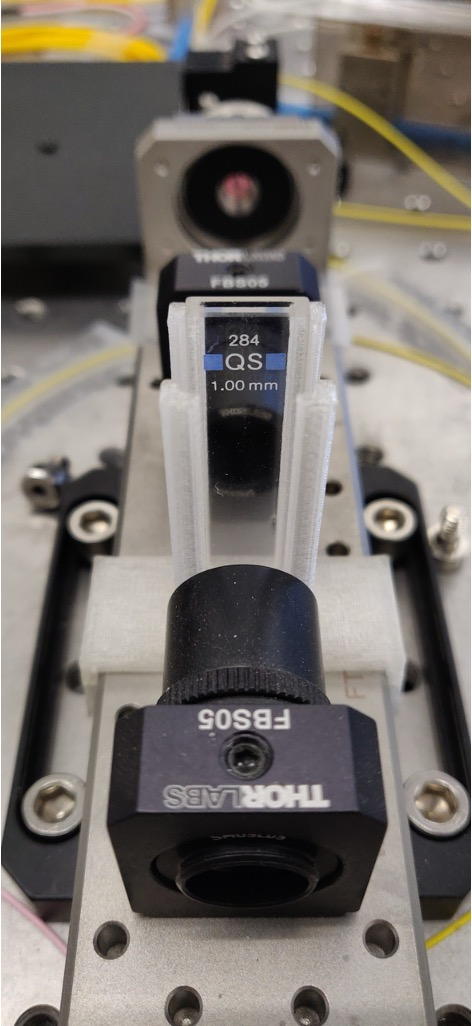
\includegraphics[width=\textwidth]{figs/4-Raman/1mmCS2.jpg}
        \label{fig:Raman:1mmCS2}
    \end{subfigure}
    \hfill
    \begin{subfigure}[b]{0.3\textwidth}
        \centering
        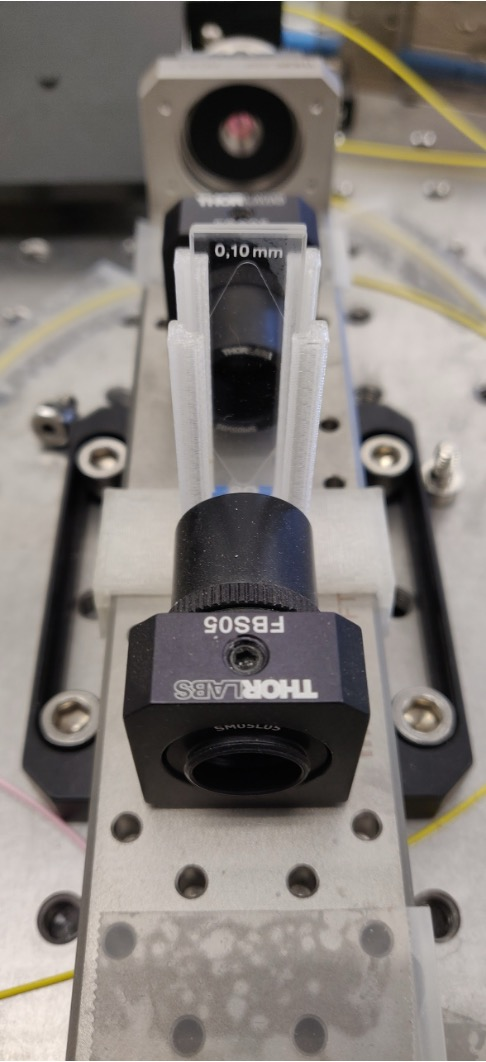
\includegraphics[width=\textwidth]{figs/4-Raman/100umCS2.jpg}
        \label{fig:Raman:100umCS2}
    \end{subfigure}
    \hfill
    \begin{subfigure}[b]{0.3\textwidth}
        \centering
        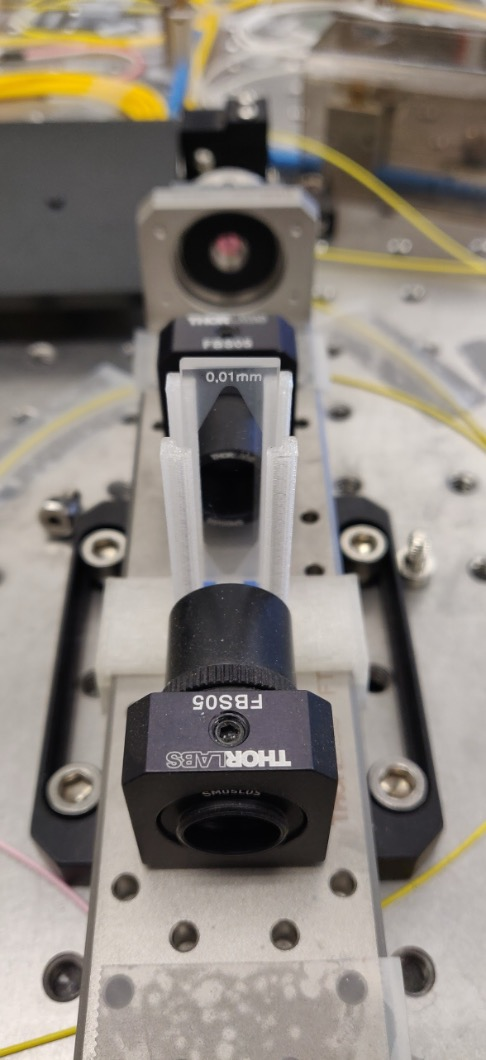
\includegraphics[width=\textwidth]{figs/4-Raman/10umCS2.jpg}
        \label{fig:Raman:10umCS2}
    \end{subfigure}
    %
    \caption{Three \ce{CS2} cells of different path lengths (\SI{1}{\milli\meter}, \SI{100}{\micro\meter}, and \SI{10}{\micro\meter}) secured in the beam path of the \acl{CoBS}.}
    \label{fig:Raman:CS2Comparison}
\end{figure}

\subsection{Suspended Silica Rib Waveguide}
\label{subsec:Raman:Target:Waveguide}

\begin{itemize}
  \item BYU collab
  \item If we can couple chip waveguide into CoBS fiber-chip-fiber, then we have access to a playground of materials and geometries
  \item initial test took 9 months to learn and measure
\end{itemize}

\subsection{Elastically-Suspended Photonic-Phononic Waveguide}
\label{subsec:Raman:Target:WigglyWaveguide}

Figure~\ref{fig:Raman:wigglyCoBSspectra} plots the spectra collected from a \ac{CoBS} measurement of backward Brillouin scattering in the elastically-suspended silica rib of the photonic-phononic waveguide. In this section, we present theoretical estimates of the key mechanical modes and optomechanical couplings predicted for the elastically-suspended photonic-phononic waveguide under development. The structure under consideration consists of a polymeric (SU-8) membrane that is tensioned during high-temperature curing and supports a rib waveguide above it. This combined membrane-and-rib geometry gives rise to multiple distinct mechanical resonances that can be excited and probed optically via the \ac{CoBS} instrument operating in the forwards scattering configuration. We summarize below the principal modes, referred to as ``drumhead'' modes for the membrane and ``breathing'' modes for the rib, and estimate rough frequency ranges in which they are expected to appear.

\begin{figure}[t]
  \centering
  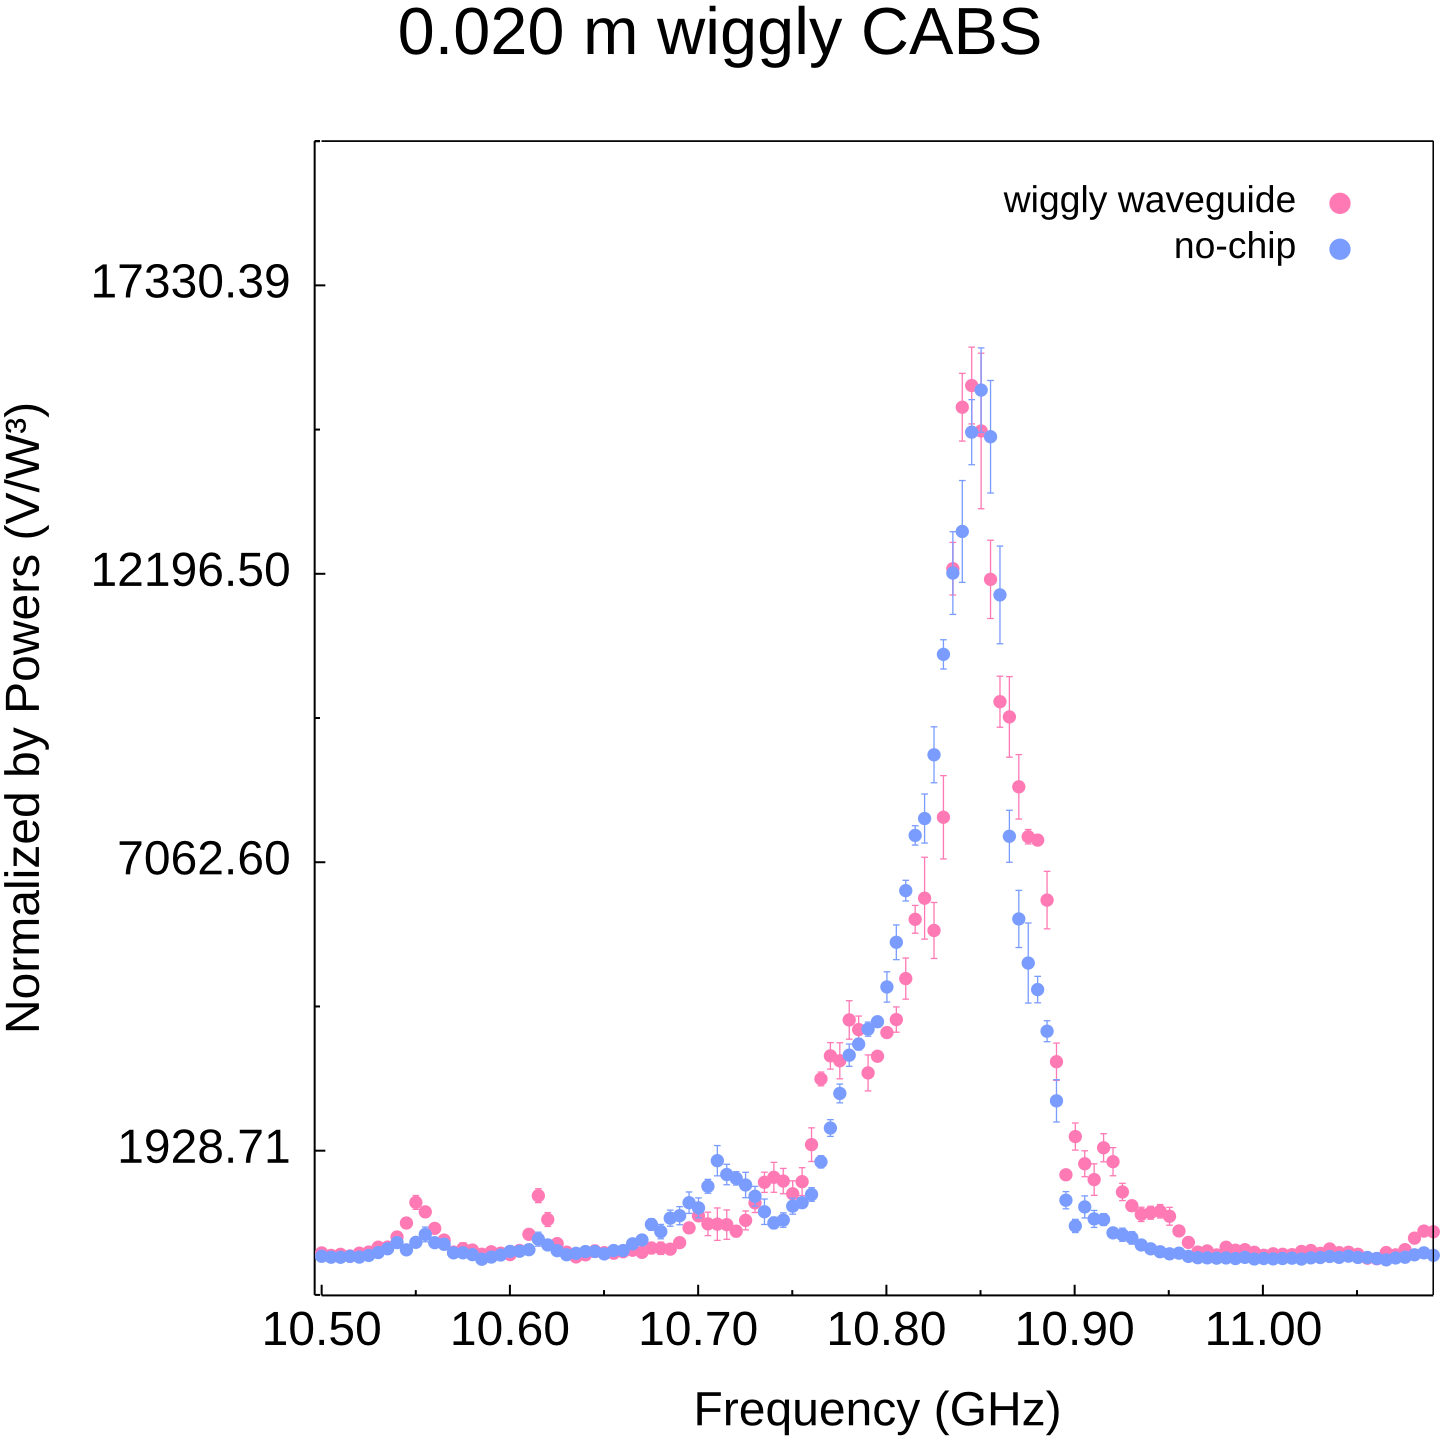
\includegraphics[width=\textwidth]{figs/4-Raman/wigglyWaveguideMeasurement.png}
  \caption{\ac{CoBS} measurement of the elastically-suspended photonic-phononic waveguide for a backward scattering process. A subsequent measurement with the chip waveguide removed reveals a similar spectral profile, as expected from the identical resonant frequency response of the \ac{SMF-28} which comprises much of the apparatus, especially in the sample region of the instrument where all three optical powers overlap. In obtaining the spectra, five repeated measurements of both the signal and background (probe off) were collected at a \SI{100}{\hertz} \ac{RBW}, dwelling for \SI{1}{\second} at each \SI{5}{\mega\hertz} frequency step. Plotted is the resulting background-subtracted spectrum. Uncertainties represent 1\(\sigma\) standard error of the mean.}
  \label{fig:Raman:wigglyCoBSspectra}
\end{figure}

We first consider the rib portion of the waveguide, having characteristic lateral width and thickness of \SI{4}{\centi\meter} and \SI{6}{\centi\meter}, respectively. One can treat the smallest cross-sectional dimension, denoted \(d\), as setting the approximate half-wavelength condition for its fundamental breathing mode. The simplest estimate for such a half-wavelength mechanical resonance is given by

\begin{equation}
f_{\rm rib,breathe} \approx \frac{v_{\rm s}}{2d},
\end{equation}
\\
where \(v_{\rm s}\) is the speed of sound in the silica rib and \(d\) is the lateral width. Taking the rib to be \SI{6}{\micro\meter} wide and assuming a speed of sound in the range \SI{5}{\kilo\meter\per\second} to \SI{6}{\kilo\meter\per\second}, this places the fundamental rib breathing mode near several hundred \si{\mega\hertz} (estimates range from \SI{400}{\mega\hertz} to \SI{500}{\mega\hertz}). Higher-order modes can arise (integer multiples of the half-wavelength condition), and so in practice one expects a series of possible breathing modes in the 100s of \si{\mega\hertz} to low-\si{\giga\hertz} range.

In principle, when optically excited via the \ac{CoBS} process, the rib breathing mode can couple to and drive displacement of the underlying membrane. Conversely, membrane motion at or near the rib’s breathing-frequency range can stimulate the rib's motion. Indeed, the waveguide design permits either the drumhead mode of the membrane or the rib breathing mode to be excited off-resonance and potentially induce mechanical vibration in the other. Beneath the rib, the polymer membrane is suspended over an open region which has been etched away, and is anchored on either side. We thus expect a classical drumhead family of modes in which the membrane oscillates out-of-plane. The tension provided by the fabrication curing process (on the order of a few tens of \si{\mega\pascal}) indicates that the membrane is tension-dominated. For a square membrane of length and width \(L\), under tension \(T\) and with mass density \(\rho\) and thickness \(h\), the fundamental frequency (1,1) can be approximated by

\begin{equation}
  f_{\rm membrane,\,drumhead\,(1,1)} \approx \frac{v_{\rm s}}{\sqrt{2}L},
  \label{eq:Raman:SquareMembrane}
\end{equation}
\\
where \(v_{\rm s}\) is the \emph{transverse} sound speed of the membrane, given by

\begin{equation}
  v_{\rm s} = \sqrt{\frac{T}{\rho h}} = \sqrt{\frac{\sigma h}{\rho h}} = \sqrt{\frac{\sigma}{\rho}},
  \label{eq:Raman:TransverseSoundSpeed}
\end{equation}
\\
where \(\sigma\) is the stress (\si{\pascal}) corresponding to the tension per membrane thickness (\(\sigma = T/h\)).

Modeling the polymer membrane as a square membrane, we can estimate the fundamental membrane drumhead mode using a mean density of SU8 (\(\rho=\)\SI{1190}{\kilo\gram\per\cubic\meter}) \cite{roch2003fabrication} and needle profilometer tension measurements performed on the membrane. Figure~\ref{fig:Raman:profilometer} plots deflection for various stylus force values applied to the membrane. The inverse of the slope of these data (taken to be linear, \(m\sim\)\SI{300}{\newton\per\meter}) allows for the membrane's approximate tension to be found via \(T=\frac{L}{4}m\sim\)\SI{2}{\milli\newton\per\meter}. For a \SI{2}{\micro\meter}-thickness with Equation~\ref{eq:Raman:TransverseSoundSpeed}, this gives an approximate transverse sound speed of a very low \(v_{\rm s}\sim\)\SI{1}{\meter\per\second}. Inserting this into Equation~\ref{eq:Raman:SquareMembrane} with length \(L\approx\)\SI{25}{\micro\meter}, we anticipate the fundamental drumhead mode resonant frequency of the SU8 membrane to lie around \SI{30}{\kilo\hertz}. Meanwhile, the rib breathing mode are predicted to lie around the mid-100s of \si{\mega\hertz}. Given this 4-order-of-magnitude discrepancy in resonant frequencies, the two mechanical modes are not expected to exhibit mechanical coupling, even when accounting for the possibility of off-resonant driving. To have the two resonances approach each other, one might alter the fabrication parameters to try significantly increasing the resulting tension of the membrane, perhaps by experimenting with different bake times or temperatures and membrane thicknesses. Alternatively, or additionally, shortening the length \(L\) across which the membrane spans from clamp-to-clamp would minimally nudge its resonant frequency higher.

\begin{figure}[t]
  \centering
  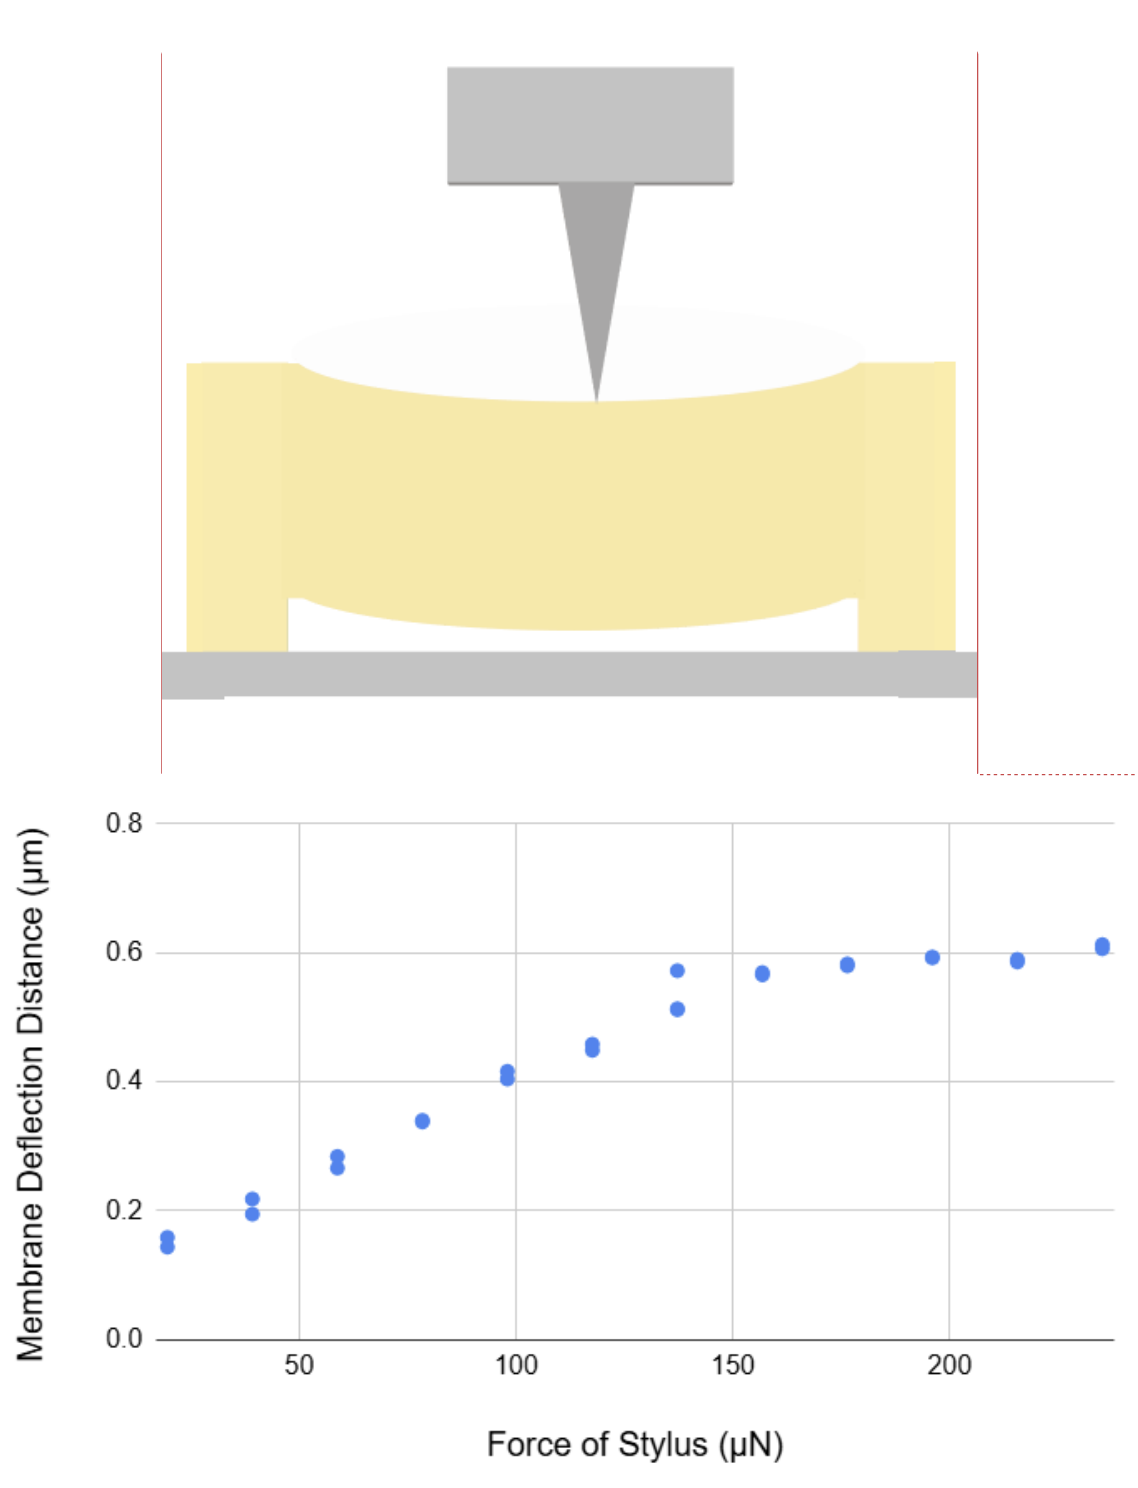
\includegraphics[width=0.7\textwidth]{figs/4-Raman/profilometer.png}
  \caption{Needle profilometer force-deflection measurements (illustrated above) performed on the suspended polymer membrane of the photonic-phononic waveguide. The inverse slope of the data (taken to be linear) is proportional to the tension of the membrane (\(m\propto T\)). Using \(m\sim\)\SI{300}{\newton\per\meter}, we estimate the tension of the membrane to be \(T\sim\)\SI{2}{\milli\newton\per\meter}, giving a very slow transverse sound speed \(v_{\rm s}\sim\)\SI{1}{\meter\per\second} via Equation~\ref{eq:Raman:TransverseSoundSpeed}.}
  \label{fig:Raman:profilometer}
\end{figure}

\begin{figure}[t]
  \centering
  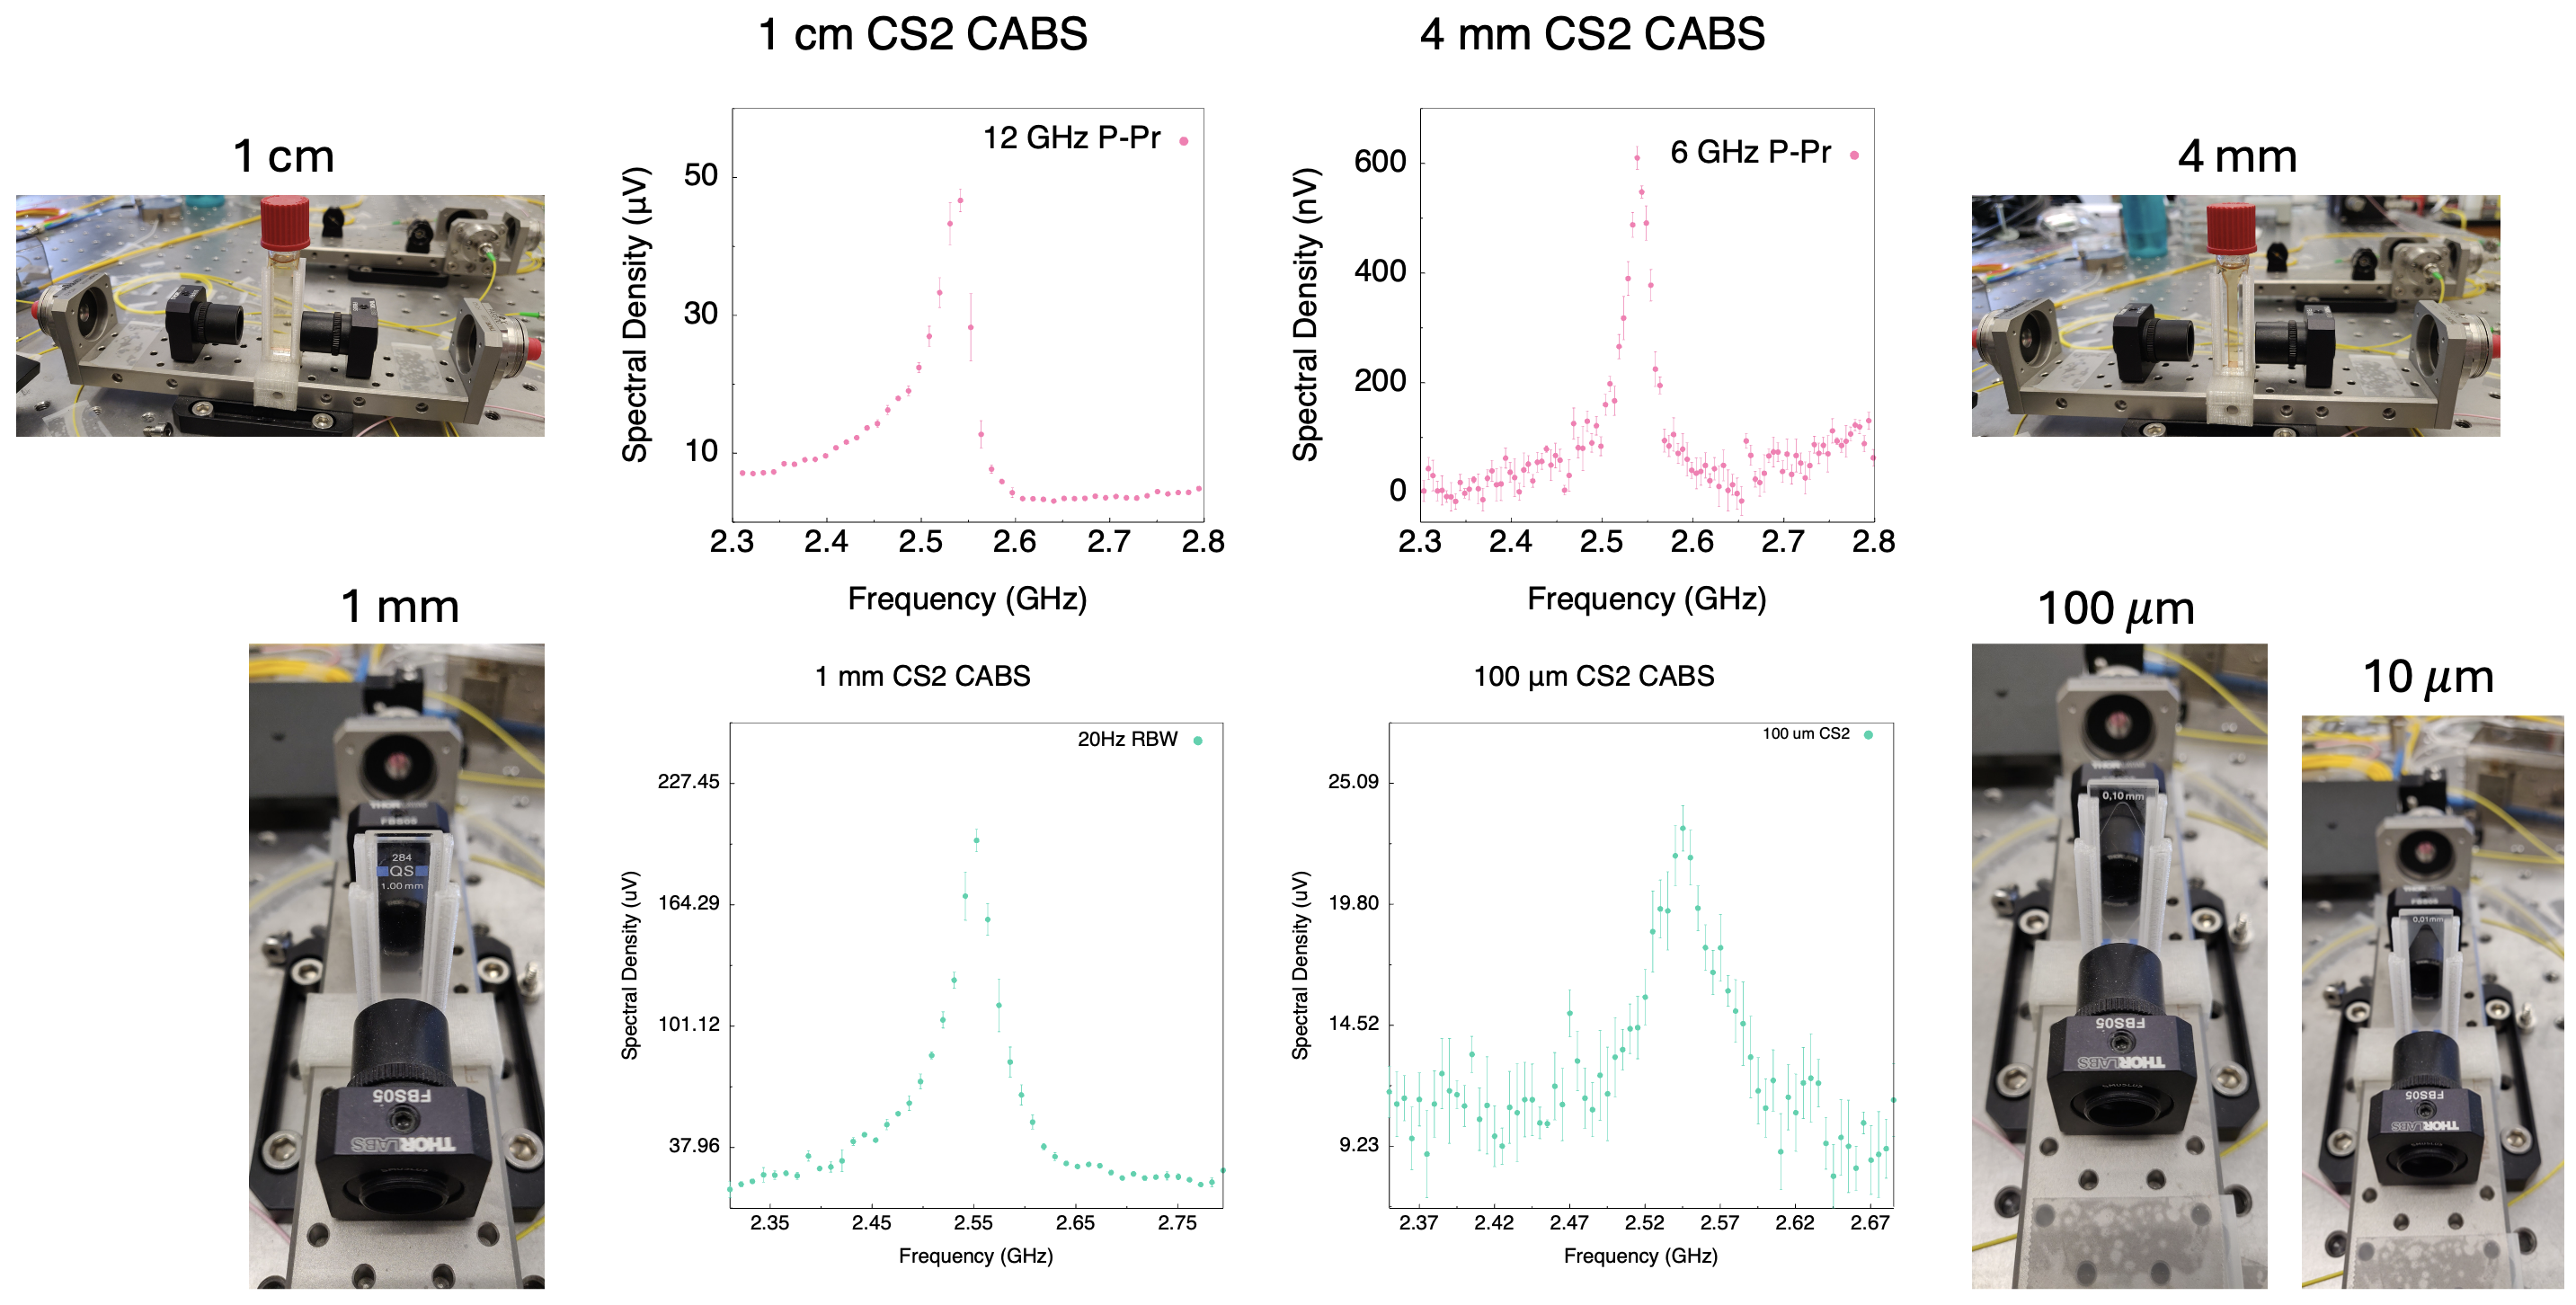
\includegraphics[width=\textwidth]{figs/4-Raman/StartBigApproachSmall.png}
  \caption{Start big, approach small.}
  \label{fig:StartBigApproachSmall}
\end{figure}

\begin{figure}[t]
  \centering
  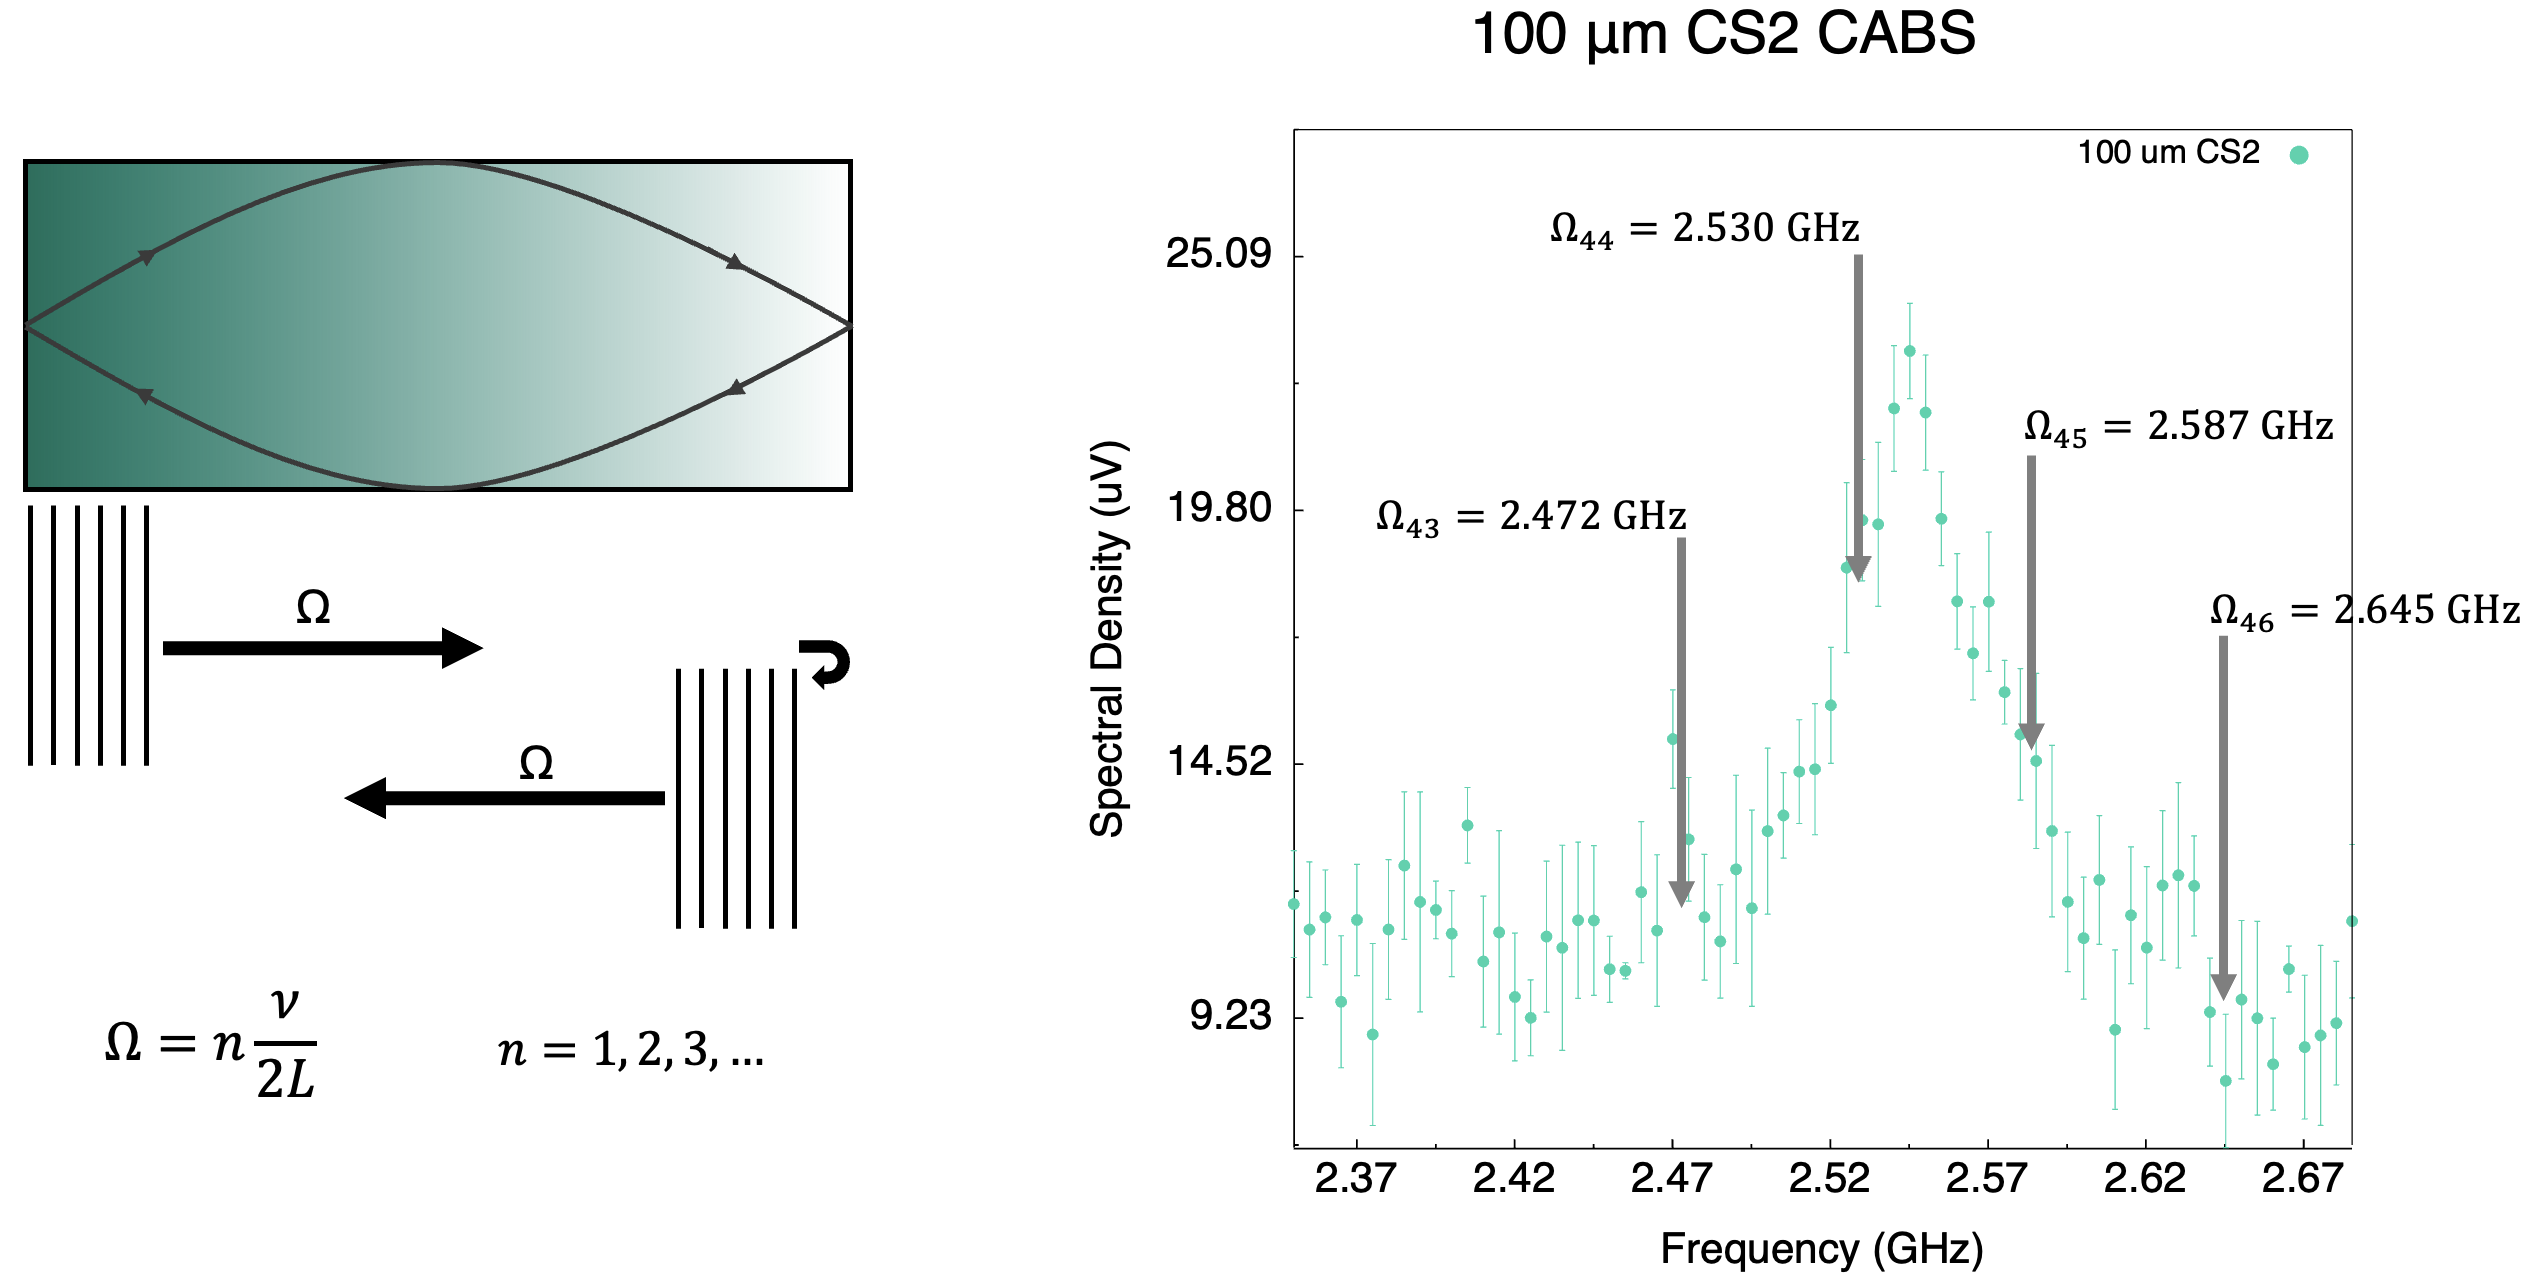
\includegraphics[width=\textwidth]{figs/4-Raman/HowWouldRamanModesAppear.png}
  \caption{How would Raman modes appear.}
  \label{fig:HowWouldRamanModesAppear}
\end{figure}

%--------------------------------------------------------------------%

\section{Discussion}
\label{sec:Raman:Discussion}

\subsection{Pathways to Brillouin-Induced Raman Modes}
\label{subsec:Raman:Pathways}

Ideal platforms by category
\begin{itemize}
  \item waveguide - long TeO2 rib, evenly spaced square holes
  \item TeO2 thin film/crystal - dissolve only small area of substrate for beam spot
  \item CS2 cell - 5um
  \item Fiber - notched, acoustic fiber Bragg grating
\end{itemize}

\subsection{Conclusion}
\label{subsec:Raman:Conclusion}

Connection to Dissertation Theme
\begin{itemize}
  \item Relate back to the broader aims of controlling phonons at room temperature, highlighting how these efforts extend exploration of optomechanical interactions.
\end{itemize}

\clearpage
\thispagestyle{empty}
\null
\newpage


%%%%%%%%%%%%%%%%%%%%%%%%%%%%%%%%%%%%%%%%%%%%%%%%%%%%%%%%%%%%%%%%%%%%%%%%%%%
% \clearpage
\setcounter{rownumber}{0}
\singlespacing
\chapter{Manuscript IV: Nanoscale Brillouin scattering}
\label{chap:chapterIV}
\acresetall

%  Copy this file for each main chapter, make sure to add it to main.tex

% Example author list with footnote style affiliations
%
% Christian J. Tai Udovicic\footnote{\label{spweather:nau}\ac{NAU}, \ac{DAPS}, PO Box 6010, Flagstaff, AZ 86011, USA}, Emily S. Costello\footnote{University of Hawai'i at Manoa, Honolulu, HI, USA}, Rebecca R. Ghent\footnote{Planetary Science Institute, Tucson, AZ, USA}, Christopher S. Edwards$^\mathrm{\ref{spweather:nau}}$

%  Extra copyright disclaimer to be safe
%
% \textit{This is the Accepted Manuscript version of an article accepted for publication in \ac{GRL}. Wiley Inc is not responsible for any errors or omissions in this version of the manuscript or any version derived from it. The Version of Record is available online at} \url{https://doi.org/10.1029/2020GL092198}\textit{.}

\doublespacing

%%%%%%%%%%%%%%%%%%%%%%%%%%%%%%%%%%%%%%%%%%%%%%%%%%%%%%%%%%%%%%%%%%%%
%  Chapter contents here

\section{Abstract}
\lipsum[2]


\section{Introduction}
\lipsum[2]

\begin{table}[htb]
\caption{Table caption.}
\centering
\begin{tabular}{l l c l}
\hline
& Parameter & Value & Description  \\
\hline
\multirow{5}{6em}{Lookup Variables}
 & lat  & -85$\degree$--85$\degree$ & Latitude (35 bins in 5$\degree$ increments)  \\
 & ALBEDO  & 0.05--0.225 & Bolometric albedo (6 bins in 0.035 increments)  \\
 & SLOPE  & 0$\degree$--90$\degree$ & Surface slope (19 bins in 5$\degree$ increments)   \\
 & SLOAZI  & 0$\degree$--360$\degree$ & Surface azimuth (19 bins in 20$\degree$ increments)   \\
 & DELLS  & 4$\degree$ & $L_s$ step size (90 bins spanning 0$\degree$--360$\degree$) \\
\hline
\multirow{8}{6em}{Thermal Parameters}
 & EMISS  & 0.96 & Emissivity  \\
 & thick  & 0.05 & Upper layer thickness [m] \\
 & DENSITY  & 1100 & Upper layer density [kg/m$^3$]  \\
 & DENS2  & 1800 & Lower layer density [kg/m$^3$]  \\
 & lbound  & 18 & Interior heat flow [mW/m$^2$]   \\
 & \multirow{3}{*}{PhotoFunc}  & \multirow{3}{*}{0.045/albedo} & \multirow{3}{20em}{Photometric function (Keihm-style)} \\
 & & & \\
 & & & \\
\hline
\multirow{12}{6em}{Temperature-dependent parameters}
 & SphUp0/SphLo0  & 602.88098583 & \multirow{4}{20em}{Specific heat capacity expressed as 4th-order polynomial ($\rm c0 + c1 \cdot T + c2 \cdot T^2 + c3 \cdot T^3$)} \\
 & SphUp1/SphLo1  & 235.98988249 &  \\
 & SphUp2/SphLo2  & -29.59742178 &  \\
 & SphUp3/SphLo3  & -3.78707193  & \\
 \\
 & ConUp0  & 0.00133644 &  \multirow{4}{20em}{Upper layer conductivity expressed as 4th-order polynomial ($\rm c0 + c1 \cdot T + c2 \cdot T^2 + c3 \cdot T^3$)} \\
 & ConUp1  & 0.00073150 &  \\
 & ConUp2  & 0.00033250 &  \\
 & ConUp3  & 0.00005038 &  \\
 \\
 & ConLo0  & 0.00634807 &  \multirow{4}{20em}{Lower layer conductivity expressed as 4th-order polynomial ($\rm c0 + c1 \cdot T + c2 \cdot T^2 + c3 \cdot T^3$)} \\
 & ConLo1  & 0.00347464 &  \\
 & ConLo2  & 0.00157938 &  \\
 & ConLo3  & 0.00023930 &  \\
\hline
\multirow{8}{6em}{Model Setup Parameters}
 & body  & Moon & Target body  \\
 & k\_style  & Moon & Conductivity style (Moon for airless bodies)  \\
 & LKofT  & T & Temperature-dependent conductivity  \\
 & FLAY  & 0.01 & First layer thickness [m]  \\
 & RLAY  & 1.3 & Layer thickness multiplier    \\
 & N1  & 26 & Number of layers  \\
 & N24  & 288 & Timesteps per day (5 min steps)  \\
 & DJUL  & 0 & Start date  \\
\hline
\end{tabular}
\label{stab:parametersIV}
\end{table}

\lipsum[2]


%%%%%%%%%%%%%%%%%%%% DISCUSSION %%%%%%%%%%%%%%%%%%%%%%%%%%%%%%%%%%%%%%%%%%%
\clearpage
\chapter{Discussion \& Future Work}
\label{chap:discussion}
\acresetall


\clearpage
\thispagestyle{empty}
\null
\newpage


%%%%%%%%%%%%%%%%%%%%%%%%%%%%%%%%%%%%%%%%%%%%%%%%%%%%%%%%%%%%%%%%%%%%%%%%%%%
\clearpage
\singlespacing
\chapter*{Acronyms}
\phantomsection
\addcontentsline{toc}{chapter}{Acronyms}
\label{chap:acronyms}
\begin{acronym}
\acro{AGU}{American Geophysical Union}
\end{acronym}


%%%%%%%%%%%%%%%%%%%%%%%%%%%%%%%%%%%%%%%%%%%%%%%%%%%%%%%%%%%%%%%%%%%%%%%%%%%
\clearpage
\doublespacing
\appendix
\chapter{Supplementary Information for Chapter \ref{chap: 2-Cooling}: Manuscript I}
\label{appendix: 2-Cooling}
\acresetall

\section{Mean-field analysis of Brillouin cooling}
\label{SI:meanField}
The key features of Brillouin cooling can be understood from a mean-field analysis of the slowly-varying envelope equations. For an undepleted pump and ignoring the propagation of phonons, spontaneous Brillouin scattering can be described by the following coupled stochastic envelope equations
\begin{eqnarray}
\label{SVE}
   && \dot{A}_S + v_g \partial_z A_S = -i g A_p B_S^\dag \\
   && \dot{B}_S + \frac{\Gamma_0}{2} B_S  = -i g A_p A_S^\dag + \xi_S \\
      \label{SVE-3}
   && \dot{A}_{aS} + v_g \partial_z A_{aS} = -i g A_p B_{aS} \\
   \label{SVE-4}
   && \dot{B}_{aS} + \frac{\Gamma_0}{2} B_{aS}  = -i g A_{aS} A_p^\dag + \xi_{aS}
\end{eqnarray}
expressed in a frame rotating at the resonance frequency for each field \cite{kharel2016noise}.
Here, $A_{S}$ ($A_{aS}$) and $B_{S}$ ($B_{aS}$) are the respective (right-moving) optical and mechanical envelopes for the Stokes (anti-Stokes) process, $A_p$ is the envelope for a constant undepleted pump, $g$ is the Brillouin coupling, and $v_g$ is the optical group velocity. Thermal fluctuations of the mechanical field are modeled using the locally correlated white noise Langevin forces
$\xi_{j}$ ($j=S$ or $aS$)  with correlation properties
\begin{eqnarray}
  &&  \langle \xi_j(t,z) \xi_{j'}^\dag(t',z')\rangle = \Gamma_0 (n_{th}+1) \delta_{jj'} \delta(t-t')\delta(z-z') \quad \quad \\
  \label{corr-2}
  && \langle \xi_j^\dag(t,z) \xi_{j'}(t',z')\rangle = \Gamma_0 n_{th} \delta_{jj'} \delta(t-t')\delta(z-z')
\end{eqnarray}
and $\Gamma_0$ is the mechanical dissipation rate. Put in terms of readily measurable quantities, the power in an optical mode is given by $P_{S/aS/p} = \hbar \omega_{S/aS/p} v_g A^\dag_{S/aS/p}A_{S/aS/p}$ and the Brillouin gain can be expressed as

\begin{equation}
\label{eq:GB}
    G_B = \frac{4 |g|^2}{\hbar \omega_p v_g^2 \Gamma_0}.
\end{equation}

We define the mean fields for the respective optical and mechanical fields $a_j$ and $b_j$  as the average of the envelope over the length of the waveguide
\begin{eqnarray}
&&  a_j = \frac{1}{L}\int_0^L dz \ A_j(z)
\\
&&  b_j = \frac{1}{L}\int_0^L dz \ B_j(z).
\end{eqnarray}

 The mean field equations can be obtained by averaging Eqs. \eqref{SVE}-\eqref{SVE-4} over the waveguide length, giving
\begin{eqnarray}
\label{eq:mean-field}
   && \dot{a}_S + \frac{\gamma}{2}a_S = -i g A_p b_S^\dag \\
   \label{eq:mean-field-2}
   && \dot{b}_S + \frac{\Gamma_0}{2} b_S  = -i g A_p a_S^\dag + \bar{\xi}_S \\
   && \dot{a}_{aS} + \frac{\gamma}{2} a_{aS} = -i g A_p b_{aS} \\
   \label{eq:mean-field-4}
   && \dot{b}_{aS} + \frac{\Gamma_0}{2} b_{aS}  = -i g a_{aS} A_p^\dag + \bar{\xi}_{aS}
\end{eqnarray}
where $\bar{\xi}_j$ is the spatial average of the Langevin force. Here, the mean-field optical decay rate $\gamma = 4 v_g/L$ is obtained from the spatial average of the derivative terms, assuming $a_j \approx (A_j(L)+A_j(0))/2$ and using that the scattered optical fields vanish at the input face, i.e., $A_j(0) = 0$, according to
\begin{eqnarray}
    \frac{v_g}{L} \int_0^L dz  \ \partial_z A_k(z)  = && \frac{v_g}{L}(A_k(L)-A_k(0)) \nonumber
   \\
    = && \frac{v_g}{L}(A_k(L)+ A_k(0)-2A_k(0))  \nonumber
   \\
    = && \frac{2v_g}{L}a_k.
\end{eqnarray}

Next we analyze the mean field dynamics. When $\gamma > \Gamma_0$, the optical fields respond to changes in the phonon amplitude faster than the phonon changes, enabling a quasistatic solution to the optical field dynamics given by
\begin{eqnarray}
\label{eq:Ad-Elim}
   &&  \frac{\gamma}{2}a_S \approx -i g A_p b_S^\dag \\
   \label{eq:Ad-Elim-2}
   &&  \frac{\gamma}{2} a_{aS} \approx -i g A_p b_{aS}.
\end{eqnarray}
Inserting Eq. \eqref{eq:Ad-Elim} \& \eqref{eq:Ad-Elim-2} into Eqs. \eqref{eq:mean-field-2} \& \eqref{eq:mean-field-4} we find the effective phonon dynamics given by
\begin{eqnarray}
\label{eq:eff-mean-field}
   && \dot{b}_S + \frac{1}{2} \Gamma_S b_S  =  \bar{\xi}_S \\
   \label{eq:eff-mean-field-2}
   && \dot{b}_{aS} + \frac{1}{2}\Gamma_{aS} b_{aS}  =  \bar{\xi}_{aS}
\end{eqnarray}
where $P_p = \hbar \omega_p v_g A^\dag_p A_p$, Eq. \eqref{eq:GB} and Eq. (2) of the main text have been used. In addition, to changing the effective phonon dynamics, these results show that the power spectra for the optical fields are proportional to the phonon power spectrum,
\begin{eqnarray}
   && \!\!\!\!\!\!\!\!\!\!S_S[\omega] = \frac{4|g|^2 |A_p|^2}{\gamma^2} \!\int_{-\infty}^{\infty} d\tau \ e^{i\omega \tau} \langle b_S(t+\tau) b_S^\dag(t)\rangle
    \\
   && \!\!\!\!\!\!\!\!\!\! S_{aS}[\omega] = \frac{4|g|^2 |A_p|^2}{\gamma^2} \!\int_{-\infty}^{\infty} d\tau \ e^{i\omega \tau} \langle b^\dag_{aS}(t\!+\!\tau) b_{aS}(t)\rangle \quad \quad
\end{eqnarray}
illustrating how the optical power spectra, defined by
$S_j[\omega] = \int_{-\infty}^{\infty} d\tau \ \exp\{i\omega\tau\} \langle a^\dag_{j}(t+\tau) a_{j}(t)\rangle$, permit a form of nonequilibrium phonon spectroscopy. Solving Eqs. \eqref{eq:eff-mean-field} and using the correlation properties for the spatially averaged Langevin forces given by
\begin{eqnarray}
  &&  \langle \bar{\xi}_j(t) \bar{\xi}_{j'}^\dag(t')\rangle = \frac{1}{L}\Gamma_0 (n_{th}+1) \delta_{jj'} \delta(t-t') \\
  && \langle \bar{\xi}_j^\dag(t) \bar{\xi}_{j'}(t')\rangle = \frac{1}{L}\Gamma_0 n_{th} \delta_{jj'} \delta(t-t'),
\end{eqnarray}
we find
\begin{eqnarray}
   && S_S[\omega] = \frac{\Gamma_0 G}{4  v_g} \frac{\Gamma_0 n_{th}}{\Gamma_S} \frac{\Gamma_S}{\omega^2 + \Gamma_S^2/4}
    \\
   && S_{aS}[\omega] = \frac{\Gamma_0 G }{4 v_g} \frac{\Gamma_0 n_{th}}{\Gamma_{aS}} \frac{\Gamma_{aS}}{\omega^2 + \Gamma_{aS}^2/4}.
\end{eqnarray}
The peak of the power spectrum (i.e., on resonance, or $\omega = 0$), used for the theory in Fig. 2e, is given by
\begin{eqnarray}
   && S^{peak}_S[P_p] = \frac{n_{th}}{v_g} \frac{GB P_p L}{(1-\frac{1}{4} G_B P_p L)^2}
    \\
   && S^{peak}_{aS}[P_p] = \frac{n_{th}}{v_g} \frac{G_B P_p L}{(1+\frac{1}{4} G_B P_p L)^2}.
\end{eqnarray}
To account for the radio-frequency to electrical conversion, the peak of the power spectrum at the lowest power ($P_0 = 4.1$ mW) is used to scale the theoretical curves to have units of $\mu V$
\begin{eqnarray}
    && S^{peak,RF}_S[P_p] = \frac{S^{peak,RF}_S[P_0]}{G_B P_0 L} \frac{G_B P_p L}{(1-\frac{1}{4} G_B P_p L)^2} \quad \quad
    \\
   && S^{peak,RF}_{aS}[P_p] = \frac{S^{peak,RF}_{aS}[P_0]}{G_B P_0 L} \frac{G_B P_p L}{(1+\frac{1}{4} G_B P_p L)^2}. \quad\quad\quad
\end{eqnarray}

\subsection{Envelope analysis of cooling dynamics, and validity of the mean-field model}
Here, we show that in the limit of small single-pass gain, the conclusions of the mean-field model agree with the full envelope dynamics.

In the Fourier domain, Eq. \eqref{SVE-4} can be readily solved and inserted in Eq. \eqref{SVE-3}, giving

\begin{eqnarray}
\label{SVE-3p}
   && (\partial_z -i \Lambda)A_{aS}(\omega,z) = -\frac{1}{v_g}i g A_p \hat{B}_{aS}(\omega,z) \quad
\end{eqnarray}
where
\begin{eqnarray}
\label{lambda}
    \Lambda = \frac{1}{v_g}\bigg[\omega + i \frac{|g|^2 |A_p|^2}{
-i\omega + \Gamma_0/2} \bigg],
\end{eqnarray}
and \begin{eqnarray}
\label{Bhat}
\hat{B}(\omega,z) = \frac{1}{
-i\omega + \Gamma_0/2} \xi(\omega,z).
\end{eqnarray}
Using Eqs. \eqref{corr-2} and \eqref{Bhat}, the solution to Eq. \eqref{SVE-3p} at the exit face of the fiber ($z=L$),
\begin{eqnarray}
    A_{aS}(\omega,L) = -i \frac{g A_p}{v_g}\int_0^{L} dz \ e^{i\Lambda(L-z)} \hat{B}(\omega,z),
\end{eqnarray}
can be directly used to obtain the power spectrum of spontaneously scattered anti-Stokes light
\begin{eqnarray}
  S_{aS,env}[\omega] &\equiv& \frac{\langle A_{aS}^\dag(\omega,L) A_{aS}(\omega',L)\rangle}{2\pi\delta(\omega-\omega')} \nonumber \\
  &=& \frac{n_{th}}{v_g}
  \bigg[
  1-e^{
  -G(\omega)} \bigg]
\end{eqnarray}
where
\begin{eqnarray}
   G(\omega) =  \frac{\Gamma^2/4}{\omega^2+\Gamma^2/4} G.
\end{eqnarray}
Noting that the power spectrum obtained directly from \eqref{SVE-3} is directly related to the effective phonon power spectrum $S_B[\omega]$
\begin{eqnarray}
 S_{aS,env}[\omega] \!\!\!& = &\!\!\! \left| \frac{g A_p}{v_g} \right|^2 \!\! \int_0^{L} \!\!\!\!\! dz\!\!\int_0^{L} \!\!\!\!\!dz'
 e^{i\frac{\omega}{v_g}(z\!-\!z')}
 \frac{\langle {B}^\dag(\omega,z) {B}(\omega',z')\rangle}{2\pi\delta(\omega-\omega')} \nonumber \\
& = &\!\!\! \left| \frac{g A_p}{v_g} \right|^2 S_B[\omega],
\end{eqnarray}
(note the power spectrum of $B$ as opposed to $\hat{B}$) we identify the anti-Stokes phonon power spectrum including the effects of optomechanical cooling
\begin{eqnarray}
\label{phonon_ps}
 S_B[\omega] = \frac{4 n_{th} L}{G \Gamma_0}(1-e^{-G(\omega)}).
\end{eqnarray}
Using $S_B[\omega]$ we can calculate the effective thermal occupation of the anti-Stokes phonon mode
\begin{eqnarray}
 n_{eff,env} & = & \frac{1}{2\pi L}\int_{-\infty}^{\infty} d \omega \ S_B[\omega]
 \\
 & = & n_{th} e^{-G/2}(I_0(G/2) + I_1(G/2))
\end{eqnarray}
where the $\omega$-integral can be expressed in terms of modified Bessel function $I_0$ and $I_1$. Moreover, the full-width at half maximum $\Gamma_{aS,env}$ can be calculated from $S_B$ using $S_B[\Gamma_{aS,env}/2]= S_B[0]/2$ giving effective anti-Stokes phonon decay rate derived from the envelope dynamics given by
\begin{eqnarray}
    \Gamma_{aS,env} = \Gamma_0\left[ \frac{G}{-\ln\left((1+e^{-G})/2\right)}-1 \right]^{1/2}.
\end{eqnarray}
In the limit of small single-pass gain $G$, these results can be compared with the mean-field model, showing agreement to order $G$ for the effective phonon decay rate and order $G^2$ for the effective thermal occupation
\begin{align}
& \!\!\!\! n_{eff}  \approx n_{th}(1-G/4+G^2/16- G^3/64 + ...) \\
& \!\!\!\! n_{eff,env}   \approx  n_{th}(1-G/4+G^2/16- 5G^3/384 + ...)  \\
& \!\!\!\! \Gamma_{aS}  =  \Gamma_0(1+G/4) \\
& \!\!\!\! \Gamma_{aS,env}  \approx  \Gamma_0(1+G/4+G^2/32+...).
\end{align}
    For the maximum single pass gain explored in this study $G < 0.3$, the results of the mean-field and envelope models agree to better than $0.25 \%$ in effective lifewidths and better than $0.007\%$ in effective thermal occupation. The above analysis is similar for the Stokes process.

\subsection{Separation of time scales required for cooling of travelling wave phonons}

For cooling of travelling wave phonons to occur, anti-Stokes photons must exit the system more rapidly than it takes for the phonon to return to equilibrium, i.e., $4 v_g/L > \Gamma_0$. While the optomechanical cooling dynamics leads to an increase in the phonon relaxation rate $\Gamma_+$ with pump power, as described by Eq. \eqref{eq:gamma}, we will show that a simultaneous increase in the anti-Stokes photon group velocity preserves the required separation of timescales. Noting that the effective anti-Stokes group velocity is given by
\begin{align}
v_{g,eff} = \left(
\frac{\partial {\rm Re}[\Lambda]}
 {\partial \omega}\right)^{-1}  \approx \left(\frac{1}{v_{g}} - \frac{G_B P_p}{\Gamma_0} \right)^{-1}
\end{align}
where $\Lambda$ is defined in Eq. \eqref{lambda} and it is assumed that $\omega$ is near resonance, i.e., $\omega \ll \Gamma_0$ \cite{okawachi2005tunable,gonzalez2005optically}, we find
\begin{align}
\frac{4 v_{g,eff}}{L} = \frac{4 v_g/L}{1- \frac{1}{4} \frac{4 v_g/L}{\Gamma_0} G}
> \Gamma_+ = \Gamma_0(1+G/4).
\end{align}
This result shows that even with the changes in the phonon decay rate produced by the cooling dynamics, the requisite separation of timescales are still satisfied  because the Brillouin nonlinearity produces a fast light effect for the participating anti-Stokes photons.

\section{Pump-probe theory}
\label{SI:pump-probe}
In this section, we develop a mean-field theory to describe the pump-probe measurements. In these measurements, both pump and probe couple to the same phonon yielding the coupled envelope equations given by
\begin{eqnarray}
\label{eq:pump-probe}
   && \dot{a}_{aS} + \frac{\gamma}{2} a_{aS} = -i g A_p b_{aS} \\
   && \dot{a}_{sig} + \frac{\gamma}{2} a_{sig} = -i g A_{pr} b_{aS} \\
   && \dot{b}_{aS} + \frac{\Gamma_0}{2} b_{aS}  = -i g a_{aS} A_p^\dag -i g a_{sig} A_{pr}^\dag + \bar{\xi}_{aS} \quad \quad
\end{eqnarray}
where $A_{aS}$ is the anti-Stokes light scattered from the pump $A_p$ and $A_{sig}$ is the anti-Stokes light scattered by the probe the undepleted probe laser $A_{pr}$.

In the quasistatic limit (i.e., $\gamma > \Gamma_0$) and assuming the $|A_p| \gg |A_{pr}|$, the effective phonon dynamics is given by Eq. \eqref{eq:eff-mean-field-2} and the power spectrum of the scattered probe light is given by
\begin{eqnarray}
\label{eq:pump-probe-power}
    S_{sig}[\omega,P_p] && \equiv \int_{-\infty}^\infty d\tau \ e^{i\omega\tau}\langle a^\dag_{sig}(t+\tau) a_{sig} (t) \rangle \nonumber  \\
   && = \frac{\Gamma_0 G_p L P_{pr} }{4 v_g} \frac{\Gamma_0 n_{th}}{\Gamma_{aS}} \frac{\Gamma_{aS}}{\omega^2 + \Gamma_{aS}^2/4}.
\end{eqnarray}
where $P_{pr}$ is the fixed probe power and $\Gamma_{aS}$ is the phonon decay rate dependent upon the pump power defined in Eq. (2) of the main text. This result shows that as $\Gamma_{aS}$ increases, i.e., with increased pump power, the power spectrum broadens and decreases in magnitude. To obtain the theoretical curve shown in Fig. 2c, we use the peak value of $S_{sig}[0,0]$ to determine the constant prefactor in Eq. \eqref{eq:pump-probe-power} where $\Gamma_{aS} \to \Gamma_0$, including the optical to radiofrequency conversion
\begin{equation}
    S_{sig}[0,0] = \frac{ G_p L P_{pr} }{ v_g} \frac{n_{th}}{\Gamma_{0}^2}.
\end{equation}
Moving out of the rotating frame yields the prediction for the scattered probe power spectrum is
\begin{eqnarray}
\label{eq:pump-probe-power-RF}
    S^{RF}_{sig}[\omega,P_p] = \frac{\Gamma_{0}^2/4}{(\omega-\omega_{pr}-\Omega)^2 + \Gamma_{aS}^2/4} S^{RF}_{sig}[0,0],
\end{eqnarray}
and used to plot the theory in Fig. 2e.

\section{Brillouin gain simulations}

We calculate the Brillouin gain spectrum by utilizing finite element simulations of the optical and acoustic modes of the LCOF. By including empirically derived material properties (see Tab. \ref{parameters}) and damping for silica \cite{vacher1981ultrasonic} and CS$_2$ \cite{coakley1975brillouin}, these simulations yield the spatial mode profiles for the electric field ${\bf E}$ and the elastic displacement ${\bf u}$ (Fig. 1c \& d). We obtain the Brillouin gain by evaluating the dissipated mechanical power using the equation
\begin{equation}
G_{B} = \frac{\omega_{\rm p}}{\Omega} \frac{1}{P_p P_S} \int_{wg} d^2x \ \langle {\bf f} \cdot \dot{\bf u} \rangle
\end{equation}
where $P_p$ and $P_S$ are the respective pump and Stokes powers of the simulated electromagnetic fields, $\Omega$ is the angular frequency of the mechanical mode, ${\bf f}$ is the electrostrictive force density, $\int_{wg}$ is an integral over the waveguide cross-section, and  $\langle  {\bf A}\cdot {\bf B} \rangle$ is the time average of the vector product ${\bf A}\cdot {\bf B}$. For propagation along the z-axis,  the electrostrictive force density ${\bf f}$ is given by
\begin{align}
\label{ }
& f_j = \frac{1}{2} \varepsilon_0 n^4 p_{ijkl} \partial_i(E_k E_l^*)
\quad {\rm (silica)}
\\
& {\bf f} = - \frac{1}{4} \varepsilon_0 \gamma_e \nabla |{\bf E}|^2 \quad ({\rm CS}_2)
\end{align}
where $\varepsilon_0$ is the permittivity of vacuum, $n$ is the refractive index, $p_{ijkl}$ is the photoelastic tensor, $\gamma_e$ is the electrostrictive constant, and the Einstein summation convention is assumed for repeated indices. In these expressions, we neglect the modal differences between the pump and the Stokes fields.

Acoustic dissipation critically determines the predicted power spectrum. We account for dissipation by including empirically obtained acoustic quality factors for silica and CS$_2$ in our simulations \cite{coakley1975brillouin,vacher1981ultrasonic}. The parameters used in our simulation are summarized in the table below.

\begin{table}[ht]
\begin{tabular}{|c|c|c|c|}
\hline material   & parameter 		& value 		            \\
\hline CS$_2$ 	& density      		&  1260   kg/m$^3$  	    \\
 		& refractive index 		&  1.5885		              \\
 		& speed of sound   		&  1226     m/s	             \\
		&electrostrictive constant ($\gamma_e$)  & 2.297   \\
  & acoustic quality factor & 23.5 \\
\hline SiO$_2$ 	&density  		     	&  2203     kg/m$^3$	     \\
 		& refractive index  		&  1.445    		    \\
 		& Young's modulus		&  73.1     GPa		    \\
 		& shear modulus   		&  31.24    GPa		    \\
 		& phot. elas. tensor (p$_{11}$,p$_{12}$,p$_{44}$) & (0.125,0.27,-0.073)   \\
   & acoustic quality factor & 1800 \\
\hline
\end{tabular}
\centering
\caption{Parameters used in simulations of spontaneous Brillouin scattering spectra.}
\label{parameters}
\end{table}

%%%%%%%%%%%%%%%%%%%%%%%%%%%%%%%%%%%%%%%%%%%%%%%%%%%%%%%%%%%%%%%%%%%%%%%%%%%
% \chapter{Supplementary Information for Chapter \ref{chap:chapter2}: Manuscript II}
% \label{appendix:chapter2}
% \acresetall


%%%%%%%%%%%%%%%%%%%%%%%%%%%%%%%%%%%%%%%%%%%%%%%%%%%%%%%%%%%%%%%%%%%%%%%%%%%
% \clearpage
\singlespacing
\renewcommand{\bibname}{References}
\phantomsection
\addcontentsline{toc}{chapter}{References}
\bibliography{references.bib}

%%%%%%%%%%%%%%%%%%%%%%%%%%%%%%%%%%%%%%%%%%%%%%%%%%%%%%%%%%%%%%%%%%%%%%%%%%%
\end{document}
